\documentclass[letterpaper,12pt]{article}
\usepackage[margin=1in]{geometry}
\usepackage{graphicx}
\usepackage{array}
\usepackage{booktabs}
\usepackage{listings}
\usepackage{xcolor}
\usepackage{amsmath}
\lstset{
    basicstyle=\ttfamily\footnotesize,
    columns=flexible,
    breaklines=true
}
% Code blocks in a smaller size, so long lines stay inside the margins.
\makeatletter
\g@addto@macro\@verbatim{\small}
\makeatother
% Let TeX loosen spacing instead of pushing long \texttt{...} into the margin.
\setlength{\emergencystretch}{3em}

\title{CS 170/CS 171: Java Programming}
\author{Zihan Liang}
\date{January 2025}

\begin{document}

\maketitle

\part{Java Basics}

\section{Data Types}
\subsection{Primitive Data Types}
\subsubsection{Primitive Data and Stack Memory}
Primitive data types are the most basic types of data available in programming languages like Java. They are not objects and are directly stored in the Stack Memory.\\
% Requires: \usepackage{array}
\begin{table}[h!]
    \centering
    \begin{tabular}{|c|c|c|c|c|}
        \hline
        \textbf{Type} & \textbf{Size} & \textbf{Default} & \textbf{Range} & \textbf{Example} \\ \hline
        \texttt{boolean} & 1 bit & \texttt{false} & \texttt{true} or \texttt{false} & \texttt{true} \\ \hline
        \texttt{char} & 2 bytes & \texttt{\textbackslash u0000} & \texttt{0} to \texttt{65,535} (Unicode) & \texttt{'A'} \\ \hline
        \texttt{byte} & 1 byte & \texttt{0} & \texttt{-128} to \texttt{127} & \texttt{100} \\ \hline
        \texttt{short} & 2 bytes & \texttt{0} & \texttt{-32,768} to \texttt{32,767} & \texttt{1500} \\ \hline
        \texttt{int} & 4 bytes & \texttt{0} & \texttt{-2,147,483,648} to \texttt{2,147,483,647} & \texttt{100000} \\ \hline
        \texttt{long} & 8 bytes & \texttt{0L} & Approx. \(\pm 9.22 \times 10^{18}\) & \texttt{1000000000L} \\ \hline
        \texttt{float} & 4 bytes & \texttt{0.0f} & Approx. \(\pm 3.40 \times 10^{38}\) & \texttt{3.14f} \\ \hline
        \texttt{double} & 8 bytes & \texttt{0.0d} & Approx. \(\pm 1.80 \times 10^{308}\) & \texttt{3.1415926} \\ \hline
    \end{tabular}
\label{tab:primitive-types}
\end{table}
\\
The stack memory is fast and is automatically allocated and deallocated when the method or block scope ends. For example:
\begin{verbatim}
public void method() {
    int x = 10;  // Stored in stack memory
    double y = 20.5;  // Stored in stack memory
}
\end{verbatim}
Here, both \texttt{x} and \texttt{y} are stored in the stack, and their memory is freed when \texttt{method()} exits.
\subsubsection{Primitive Data Exceptions}
While primitives declared inside a method or block are stored in the stack memory, primitives that are part of objects are stored in the heap memory. Why? Because the object itself resides in the heap memory.
\begin{verbatim}
class Example {
    int number;  // Stored in heap memory as part of the object
}

Example obj = new Example(); // `obj` is a reference stored in the stack,
// but the `number` field is part of the object stored in heap memory.
\end{verbatim}

\subsection{Reference Data Types}
In Java, reference data types are used to store references (memory addresses) to objects. They differ significantly from primitive data types, which store values directly. A reference data type refers to objects or arrays and stores \textbf{the memory address of the object it points to}, rather than the actual data. It means that the reference (address) is stored in the stack and the object or array itself is stored in the heap.\\
\textbf{Class Types: }A class is a blueprint for creating objects. Reference types created from classes store references to these objects.
\begin{verbatim}
class Person {
    String name;
    int age;
}

Person person = new Person(); // 'person' is a reference in heap memory.
person.name = "John";
person.age = 30;
\end{verbatim}
\textbf{String:} String is a commonly used reference data type in Java. It is immutable, meaning its value cannot be changed once created. Here, greeting is a reference to a String object stored in the heap.
\begin{verbatim}
String greeting = "Hello, World!";
\end{verbatim}
\textbf{Array: }Arrays in Java are also reference types. Even though they store primitive or reference values, the array itself is a reference to a memory location.
\begin{verbatim}
int[] numbers = {1, 2, 3, 4, 5};
// 'numbers' refers to an array object in the heap.
\end{verbatim}
\textbf{Interfaces: }Reference types can also point to objects that implement a specific interface.
\begin{verbatim}
List<String> names = new ArrayList<>();
// 'names' refers to an object of ArrayList.
\end{verbatim}

\section{Variables}
\subsection{Key Characteristics of Variables}
A variable is a location in memory used to store a data value. It has three components.
\begin{enumerate}
    \item Type: Defines the kind of data (e.g., \texttt{int}, \texttt{double}, \texttt{String}) the variable can hold.
    \item Name: The identifier or label used to reference the variable.
    \item Value: The actual data stored in the variable.
\end{enumerate}
\subsection{Variable Declaration and Initialization}
Declaring a variable involves specifying its type and name. It instructs the compiler to allocate memory for the variable.
\begin{verbatim}
type variableName;
int a; // Declares an integer variable named 'a'
\end{verbatim}
Initialization assigns a value to the variable. Variables can be initialized during declaration or later in the program.
\begin{verbatim}
type variableName = value;
int a = 10; // Declares and initializes 'a' with the value 10
\end{verbatim}
Delayed Initialization:
\begin{verbatim}
int a; // Declaration
a = 20; // Initialization
\end{verbatim}
\subsection{Rules for Using Variables}
A variable \textbf{must be declared} before it is used.\\
A variable \textbf{must be initialized} before its value is accessed.\\
Variable names should follow \textbf{naming conventions}:
\begin{enumerate}
    \item Must start with a letter or underscore.
    \item Cannot use reserved keywords.
    \item Use camelCase for readability (\texttt{exampleVariable}).
\end{enumerate}
\subsection{Types of Variables in Java}
\textbf{Local Variables: }Declared within a method or block. Accessible only within that method or block. No default value (must be initialized explicitly).\\
\textbf{Instance Variables: }Declared in a class but outside any method or block. Belong to an instance of the class (each object gets its copy). Default values are assigned (0 for integers, null for objects, etc.).\\
\textbf{Static Variables:} Declared with the static keyword. Shared across all instances of the class. Have a single memory location.\\
\textbf{Variable Scope: }Scope refers to the part of the program where the variable is accessible.
\begin{itemize}
    \item Local variables: Limited to the method/block where they are declared.
    \item Instance variables: Accessible within the class using the object reference.
    \item Static variables: Accessible using the class name.
\end{itemize}
Example:
\begin{verbatim}
public class VariableExample {
    int instanceVariable = 30; // Instance variable

    static int staticVariable = 50; // Static variable

    public void methodExample() {
        int localVariable = 10; // Local variable
        System.out.println("Local: " + localVariable);
    }

    public static void main(String[] args) {
        VariableExample obj = new VariableExample();
        obj.methodExample();

        System.out.println("Instance: " + obj.instanceVariable);
        System.out.println("Static: " + staticVariable);
    }
}
\end{verbatim}
In the example, we have an instance variable instanceVariable with a value of 30 and a static variable staticVariable with a value of 50. To access the instance variable, we need to create an object obj and use obj.instanceVariable to print its value.\\
For the static variable, we can access it directly using the class name (e.g., VariableExample.staticVariable) or through an object (e.g., obj.staticVariable). However, using the class name is recommended for clarity.\\
For the local variable localVariable, it is defined within the method methodExample. We call methodExample using the object obj to execute the method, and the local variable is printed inside the method. Local variables cannot be accessed outside their method.

\section{Operations}
\subsection{Arithmetic Operations}
Arithmetic operations are performed on numerical data types (\texttt{int}, \texttt{float}, \texttt{double}, etc.).
\begin{center}
\noindent
\begin{tabular}{|c|c|}
    \hline
    \textbf{Operator} & \textbf{Meaning} \\ \hline
    \texttt{+} & Addition \\ \hline
    \texttt{-} & Subtraction \\ \hline
    \texttt{*} & Multiplication \\ \hline
    \texttt{/} & Division \\ \hline
    \texttt{\%} & Modulus (remainder) \\ \hline
\end{tabular}
\end{center}
\texttt{char} Arithmetic: Arithmetic operations on char types are based on their ASCII values. For example, A + 1 results in the ASCII value of A (65) plus 1, producing 66.\\
\texttt{String} Concatenation: The + operator is used for concatenating strings. For example:
\begin{verbatim}
String greeting = "Hello" + " World!"; // Result: "Hello World!"
\end{verbatim}
\subsection{Logical Operations}
Logical operations are performed on boolean values (\texttt{true} or \texttt{false}).
\begin{center}
\noindent
\begin{tabular}{|c|c|}
    \hline
    \textbf{Operator} & \textbf{Meaning} \\ \hline
    \texttt{\&\&} & Logical AND \\ \hline
    \texttt{||} & Logical OR \\ \hline
    \texttt{!} & Logical NOT \\ \hline
    \texttt{>} & Greater than \\ \hline
    \texttt{<} & Less than \\ \hline
    \texttt{>=} & Greater than or equal to \\ \hline
    \texttt{<=} & Less than or equal to \\ \hline
    \texttt{==} & Equal to \\ \hline
    \texttt{!=} & Not equal to \\ \hline
\end{tabular}
\end{center}
These are primarily used for comparisons and boolean logic in conditional statements (e.g., \texttt{if}, \texttt{while}, \texttt{for}).
\subsection{Assignment Operations}
Assignment operators assign values to variables.
\begin{center}
\noindent
\begin{tabular}{|c|c|}
    \hline
    \textbf{Operator} & \textbf{Meaning} \\ \hline
    \texttt{=} & Assigns a value \\ \hline
    \texttt{+=} & Adds to the current value and assigns \\ \hline
    \texttt{-=} & Subtracts from the current value and assigns \\ \hline
    \texttt{*=} & Multiplies the current value and assigns \\ \hline
    \texttt{/=} & Divides the current value and assigns \\ \hline
    \texttt{\%=} & Computes the remainder and assigns \\ \hline
\end{tabular}
\end{center}
Here is an example.
\begin{verbatim}
int x = 10;
x += 5; // Equivalent to: x = x + 5; Result: x = 15
\end{verbatim}
\subsection{Increment and Decrement Operations}
\begin{center}
\noindent
\begin{tabular}{|c|c|}
    \hline
    \textbf{Operator} & \textbf{Meaning} \\ \hline
    \texttt{n++} & Post-increment (use \texttt{n} first, then increase by 1) \\ \hline
    \texttt{n--} & Post-decrement (use \texttt{n} first, then decrease by 1) \\ \hline
    \texttt{++n} & Pre-increment (increase \texttt{n} first, then use it) \\ \hline
    \texttt{--n} & Pre-decrement (decrease \texttt{n} first, then use it) \\ \hline
\end{tabular}
\end{center}
Here are some examples.
\begin{verbatim}
int i = 10;
int newNum = 10 * (i++); // newNum = 100, then i = 11
int j = 10;
int newNum1 = 10 * (++j); // j = 11, then newNum1 = 110
\end{verbatim}

\section{String}
\subsection{String Declaration and Initialization}
In Java, Strings are a commonly used reference data type that represents a sequence of characters. Strings in Java are immutable, meaning once created, their value cannot be changed. For string declaration and initialization, there are two different methods.\\
\textbf{Syntax 1:} Using String Literals
\begin{verbatim}
String str = "hiiiiiiiii";
\end{verbatim}
Strings can be directly assigned using double quotes. When a string literal is used, it is stored in the \textbf{String pool} to save memory.\\
\textbf{Syntax 2:} Using the new Keyword
\begin{verbatim}
String str1 = new String("hi");
\end{verbatim}
This explicitly creates a new String object \textbf{in the heap memory}, bypassing the String pool. It is less common in practice because \textbf{using literals is more memory-efficient}.

\subsection{Commonly Used String Methods}
\texttt{length()}: Returns the length of the string, i.e., the number of characters in it. In this case, \texttt{str.length()} will return 10 because \texttt{hiiiiiiiii} has 10 characters.
\begin{verbatim}
int i = str.length();
\end{verbatim}
\texttt{substring()}: Extracts a portion of the string based on indices. There are two syntaxes for \texttt{substring()}.\\
Syntax 1: \texttt{str.substring(startIndex, endIndex)} extracts characters from \texttt{startIndex} (inclusive) to \texttt{endIndex} (exclusive). For example, \texttt{str.substring(1, 2)} extracts the second character, \texttt{i}.\\
Syntax 2: \texttt{str.substring(startIndex)} extracts from \texttt{startIndex} to the end of the string. For example, \texttt{str.substring(1)} extracts \texttt{iiiiiiiii}.
\begin{verbatim}
str1 = str.substring(1, 2); // Syntax 1
str1 = str.substring(1);    // Syntax 2
\end{verbatim}
\texttt{indexOf()}: Finds the \textbf{first occurrence} of the specified substring in the string. Returns the index of the first character of the substring, or \texttt{-1} if it is not found. For example, \texttt{str.indexOf("ii")} returns 1 because the substring \texttt{ii} first appears starting at index 1.
\begin{verbatim}
int j = str.indexOf("ii");
\end{verbatim}
\texttt{equals()}: Compares the \texttt{str} and \texttt{str1} for exact equality. Returns \texttt{true} if the strings are exactly the same (case-sensitive); otherwise, returns \texttt{false}. For example, if \texttt{str = hiiiiiiiii} and \texttt{str1 = hi}, \texttt{str.equals(str1)} will return \texttt{false}.
\begin{verbatim}
boolean k = str.equals(str1);
\end{verbatim}
\texttt{compareTo()}: Compare the order of occurrence of each character in the ASCII table of the calling string and the string enclosed in parentheses. Returns:
\begin{itemize}
    \item A positive integer if the calling string (\texttt{str}) is lexicographically greater.
    \item A negative integer if the calling string is lexicographically smaller.
    \item \texttt{0} if both strings are identical.
\end{itemize}
For example, if \texttt{str = hiiiiiiiii} and \texttt{str1 = hi}, \texttt{str.compareTo(str1)} will return a positive value because \texttt{hiiiiiiiii} is lexicographically greater than \texttt{hi}.
\begin{verbatim}
int h = str.compareTo(str1);
\end{verbatim}

\subsection{Key Characteristics of Strings in Java}
\textbf{Immutable:} Strings cannot be modified once created. Any operation that appears to modify a string actually creates a new string. For example, \texttt{str.substring(1)} does not modify str but creates a new string.\\
\textbf{Stored in String Pool:} Strings created using literals are stored in a special memory region called the String pool. This improves memory efficiency.

\section{Array}
\subsection{One-Dimensional Arrays (1D Arrays)}
Arrays in Java are a collection of elements of the same data type, stored in contiguous memory locations. Arrays are fixed in size once created and provide efficient access to elements through indexing. For 1D array declaration and initialization, there are two different methods.\\
\textbf{Syntax 1:} Declare and Initialize Separately
\begin{verbatim}
int[] arr1;        // Declare
arr1 = new int[5]; // Allocate memory for 5 integers
arr1[0] = 1;       // Initialize first element to 1
arr1[1] = 2;       // Initialize second element to 2
arr1[2] = 3;       // Initialize third element to 3
\end{verbatim}
If elements are not explicitly initialized, they default to \texttt{0} for numeric types.\\
\textbf{Syntax 2:} Declare and Initialize Together
\begin{verbatim}
int[] arr2 = {1, 2, 3, 4, 5}; // Declare and initialize with values
\end{verbatim}
\textbf{Accessing Elements:} Array indices start at \texttt{0}. Accessing an element outside the valid range (e.g., \texttt{arr1[5]}) throws an \texttt{ArrayIndexOutOfBoundsException}.
\begin{verbatim}
int i = arr1[0]; // Access the first element (index 0)
\end{verbatim}
\textbf{Array Length:} The \texttt{length} property gives the total number of elements in the array. For \texttt{arr1}, \texttt{arr1.length} returns 5.
\begin{verbatim}
int j = arr1.length;
\end{verbatim}
\textbf{Fixed Size: }Arrays in Java are fixed in size, meaning you cannot add or remove elements after creation. If you need a resizable array, consider using a List (e.g., \texttt{ArrayList}).

\subsection{Two-Dimensional Arrays (2D Arrays)}
2D arrays are essentially \textbf{arrays of arrays}, where each element is itself an \textbf{array}. For 2D array declaration and initialization, there are two different methods.\\
\textbf{Syntax 1:} Declare and Initialize Together
\begin{verbatim}
int[][] arr3 = {
    {1, 2, 3}, // First row
    {2, 3, 4}  // Second row
};
\end{verbatim}
The above creates a 2D array with 2 rows and 3 columns.\\
\textbf{Syntax 2:} Declare First, Initialize Later
\begin{verbatim}
int[][] arr7 = new int[5][2]; // Allocate memory for a 5x2 array
arr7[0][0] = 1;              // Assign value to the first row, first column
arr7[1][1] = 2;              // Assign value to the second row, second column
\end{verbatim}
\textbf{Accessing Elements:} Indices for rows and columns both start at 0. For example, \texttt{arr3[0][1]} accesses the second element of the first row (value = \texttt{2}).
\begin{verbatim}
int k = arr3[0][0];
// Access the element at the first row, first column (value = 1)
\end{verbatim}

\subsection{Key Characteristics of Arrays in Java}
\textbf{Fixed Size:} Arrays cannot be resized after creation.\\
\textbf{Default Values:}
\begin{itemize}
    \item Numeric types (e.g., int, double): 0
    \item boolean: false
    \item String and other objects: null
\end{itemize}
\textbf{Length Property:} Use \texttt{.length} to get the size of the array.\\
\textbf{Multi-Dimensional Arrays:} Java supports arrays of higher dimensions, such as 3D arrays, though they are less common.

\part{Control Flow and Recursion}

\section{If-Else Statements}
\subsection{Structure of If-Else Statements}
The If-Else statement is a fundamental control structure in Java, used to execute different blocks of code based on conditions.\\
\textbf{If Statement:} Evaluates a Boolean expression. If the expression is \textbf{true}, the code block inside the \texttt{if} statement is executed. If the expression is \textbf{false}, the code block is skipped.
\begin{verbatim}
if (condition) {
    // Code block to execute if condition is true
}
\end{verbatim}
\textbf{If-Else Statement:} Provides an alternative code block to execute when the condition is false.
\begin{verbatim}
if (condition) {
    // Code block to execute if condition is true
} else {
    // Code block to execute if condition is false
}
\end{verbatim}
\textbf{If-Else If Ladder:} Evaluates multiple conditions sequentially. Once a true condition is found, its code block is executed, and the rest are skipped. If none of the conditions are true, the else block (if present) executes.
\begin{verbatim}
if (condition1) {
    // Code block for condition1
} else if (condition2) {
    // Code block for condition2
} else {
    // Default code block if no conditions are true
}
\end{verbatim}
\subsection{Example}
Comparison of Two Numbers \texttt{x} and \texttt{y}.
\begin{verbatim}
if (x > y) {
    System.out.println("x is larger");
} else if (y > x) {
    System.out.println("y is larger");
} else {
    System.out.println("x and y are equal");
}
\end{verbatim}
The output is
\begin{itemize}
    \item \texttt{"x is larger"} if \texttt{x > y}.
    \item \texttt{"y is larger"} if \texttt{y > x}.
    \item \texttt{"x and y are equal"} if neither condition is true.
\end{itemize}
\subsection{Key Points}
\textbf{Conditions:} Conditions in If-Else statements must evaluate to a Boolean value (\texttt{true} or \texttt{false}).\\
\textbf{Single Execution:} Only one block of code is executed in an If-Else If ladder.\\
\textbf{Default Block:} The \texttt{else} block is optional but executes if no conditions are true.\\
\textbf{Nesting:} If-Else statements can be nested for more complex logic.
\subsection{Flowchart of Nested if Statement}
\begin{figure}[h]
    \centering
    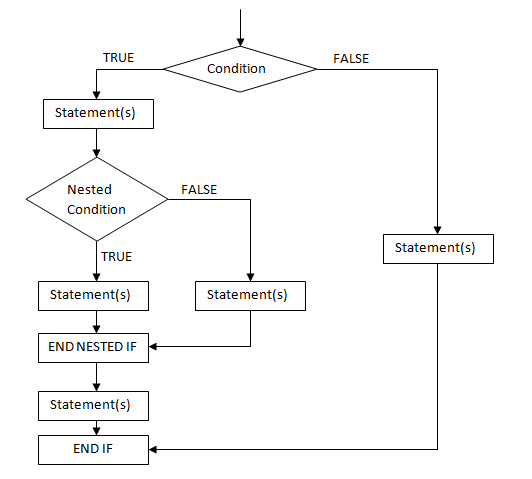
\includegraphics[width=0.5\textwidth]{nested-if_0.png}
    \caption{Flowchart of nested if statement}
\end{figure}

\section{For Loop}
\subsection{Structure of a For Loop}
\begin{verbatim}
for (initialization; condition; increment/decrement) {
    // Body of the loop
}
\end{verbatim}
\textbf{Initialization:} This is executed once at the start of the loop. It typically initializes a loop control variable.\\
\textbf{Condition:} A Boolean expression that is checked before each iteration. If the condition evaluates to \texttt{true}, the loop body executes. If \texttt{false}, the loop terminates.\\
\textbf{Increment/Decrement:} This step is executed after the body of the loop. It updates the loop control variable.
\subsection{Example of A For Loop}
\begin{verbatim}
for (int i = 0; i < 10; i++) {
    System.out.println("i = " + i);
}
\end{verbatim}
\textbf{Initialization \texttt{int i = 0}:} A loop control variable \texttt{i} is initialized to \texttt{0}.\\
\textbf{Condition \texttt{i < 10}:} As long as \texttt{i} is less than \texttt{10}, the loop will execute.\\
\textbf{Body \texttt{System.out.println("i = " + i);}:} The current value of \texttt{i} is printed to the console.\\
\textbf{Increment \texttt{i++}:} The value of \texttt{i} is increased by \texttt{1} after each iteration.
\subsection{Execution Flow}
The execution of a \texttt{for} loop follows these steps:
\begin{itemize}
    \item Initialization: The loop control variable is initialized (e.g., \texttt{int i = 0}).
    \item Condition Check: The condition is evaluated (e.g., \texttt{i < 10}). If \texttt{true}, proceed to the body of the loop. If \texttt{false}, exit the loop.
    \item Body Execution: The statements inside the loop body are executed.
    \item Increment/Decrement: The loop control variable is updated.
    \item Repeat: Steps 2–4 repeat until the condition evaluates to \texttt{false}.
\end{itemize}
\begin{figure}[h]
    \centering
    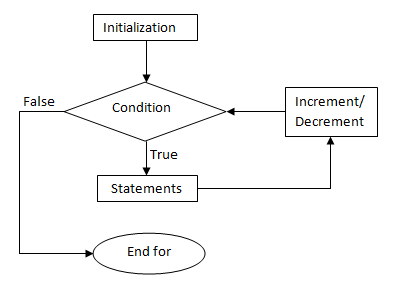
\includegraphics[width=0.5\textwidth]{for_0.png}
    \caption{Flowchart of for loop}
\end{figure}
\subsection{Characteristics of For Loops}
\textbf{Fixed Iterations:} Ideal when the number of iterations is known beforehand. For example, Loop through numbers \texttt{0-9}.\\
\textbf{Compact Syntax:} Combines initialization, condition, and increment in one line for clarity.\\
\textbf{Nested Loops:} A \texttt{for} loop can be placed inside another \texttt{for} loop for multi-dimensional iterations (e.g., iterating over a 2D array).
\subsection{Practical Usage}
\textbf{Iterating Through Arrays: }Iterates through each element of the array \texttt{arr}.
\begin{verbatim}
int[] arr = {1, 2, 3, 4, 5};
for (int i = 0; i < arr.length; i++) {
    System.out.println(arr[i]);
}
\end{verbatim}
\textbf{Counting Backward:} Prints numbers from \texttt{10 to 1}.
\begin{verbatim}
for (int i = 10; i > 0; i--) {
    System.out.println(i);
}
\end{verbatim}
\textbf{Nested Loops:} Iterates over all combinations of \texttt{i} and \texttt{j} values in a 3x3 grid.
\begin{verbatim}
for (int i = 0; i < 3; i++) {
    for (int j = 0; j < 3; j++) {
        System.out.println("i = " + i + ", j = " + j);
    }
}
\end{verbatim}

\section{While Loop}
\subsection{Structure of a While Loop}
A while loop in programming is a control flow statement that allows a block of code to be executed repeatedly based on a given Boolean condition. The execution continues until the condition evaluates to \texttt{false}.\\
\begin{verbatim}
int i = 0;
while(i < 10){
    i++;
}
\end{verbatim}
The loop starts by evaluating the condition (\texttt{i < 10}). If the condition is true, the statements inside the loop execute. The loop then re-evaluates the condition. Once the condition becomes false, the loop terminates.
\subsection{Breakdown of While Loop Execution}
\textbf{Condition Evaluation:} The loop checks whether the condition (i < 10) is true or false. If true, execution enters the loop body. If false, execution skips the loop and continues with the rest of the program.\\
\textbf{Loop Body Execution:} The code inside the while block runs (e.g., i++ in the example). The increment step ensures i increases each iteration.\\
\textbf{Rechecking Condition:} After executing the body, the condition is checked again. If still true, another iteration begins. If false, the loop terminates.
\subsection{Flowchart Representation}
\begin{figure}[h]
    \centering
    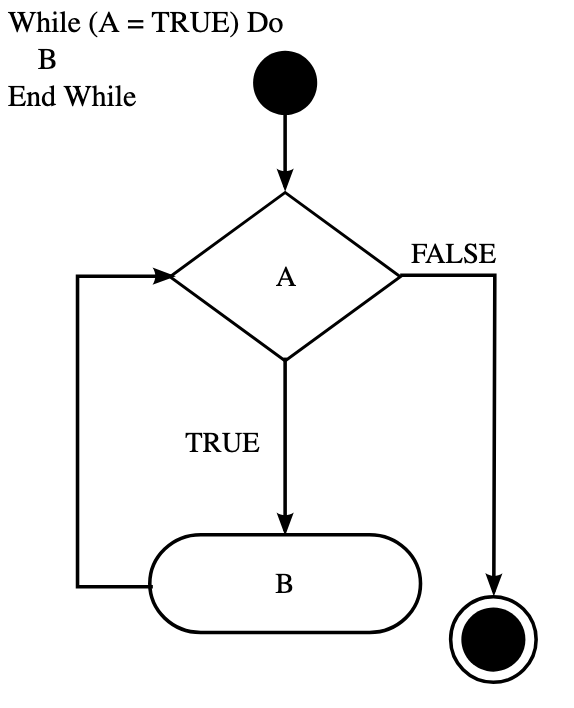
\includegraphics[width=0.4\textwidth]{while_loop.png}
    \caption{Flowchart of while loop}
\end{figure}
\subsection{Key Characteristics of While Loops}
\textbf{Pre-check loop:} The condition is evaluated before executing the loop body.\\
\textbf{Infinite loop risk:} If the condition never becomes false, the loop runs indefinitely.\\
\textbf{Used when the number of iterations is unknown:} Unlike a for loop, while loops are ideal when we do not know in advance how many times the loop should run.\\
\textbf{For loop and while loop:} All for loops can be rewritten as while loops, because both loops serve the same fundamental purpose — executing a block of code repeatedly based on a condition.

\section{Do-While Loops}
\subsection{Structure of a Do-While Loop}
\begin{verbatim}
do {
    // Code block (executed at least once)
} while (condition);
\end{verbatim}
The do-while loop is a type of loop in Java that ensures the loop body executes at least once, regardless of the condition. A do-while loop consists of two parts:
\begin{itemize}
    \item Body: Executes at least once.
    \item Condition: Checked after the body execution. If \texttt{true}, the loop runs again; if \texttt{false}, the loop stops.
\end{itemize}
The body inside \{ \} executes at least once. After execution, the condition inside \texttt{while(condition)}; is checked. If \texttt{true}, the loop runs again; if \texttt{false}, the loop stops.
\subsection{Key Differences from While Loop}

\begin{center}
\begin{tabular}{|l|l|l|}
\hline
\textbf{Feature} & \textbf{While Loop} & \textbf{Do-While Loop} \\ \hline
Execution Before Condition Check & No & Yes \\ \hline
Executes at Least Once? & No & Yes \\ \hline
Condition Check Location & Before loop body & After loop body \\ \hline
\end{tabular}
\end{center}
When the loop must run at least once (e.g., menu selection, user input validation). Example: Asking users for input at least once, then checking if they want to continue.
\begin{verbatim}
Scanner scanner = new Scanner(System.in);
int number;
do {
    System.out.println("Enter a number (0 to stop): ");
    number = scanner.nextInt();
} while (number != 0);
\end{verbatim}

\section{Which Loop?}
\subsection{Comparison of For Loop, While Loop, and Do While Loop}

\begin{center}
    \renewcommand{\arraystretch}{1.5}
    \setlength{\tabcolsep}{3pt}
    \resizebox{\textwidth}{!}{
    \begin{tabular}{|m{3cm}|m{5cm}|m{5cm}|m{5cm}|}
        \hline
        \textbf{Feature} & \textbf{For Loop} & \textbf{While Loop} & \textbf{Do While Loop} \\
        \hline
        Execution Condition & Condition is checked before each iteration & Condition is checked before each iteration & Condition is checked after each iteration \\
        \hline
        Initialization & Usually includes initialization in the loop statement & Initialization occurs before the loop & Initialization occurs before the loop \\
        \hline
        Use Case & Used when the number of iterations is known beforehand & Used when the number of iterations is unknown but the condition must be met before entering the loop & Used when at least one iteration must be executed regardless of the condition \\
        \hline
        Guarantee of Execution & May not execute if the condition is false initially & May not execute if the condition is false initially & Always executes at least once \\
        \hline
    \end{tabular}
    }
\end{center}
\subsection{General Rules}
\textbf{for loop: }known number of repetitions.\\
\textbf{while loop: }unknown number of repetitions.\\
\textbf{do-while loop: }loop body should be executed before condition check.

\section{Recursion}
Recursion is a fundamental concept in Java where a method calls itself to solve a problem. This approach is commonly used for problems that can be divided into smaller subproblems of the same type. A recursive function typically consists of two main parts:
\begin{itemize}
    \item \textbf{Base Case:} The condition under which the recursion stops.
    \item \textbf{Recursive Case:} The function calls itself with a smaller input to approach the base case.
\end{itemize}
\subsection{Example: Factorial Calculation}
A classic example of recursion is the computation of factorial, defined as:
$$
    n! = \begin{cases} 
        1, & \text{if } n = 0 \\ 
        n \times (n-1)!, & \text{if } n > 0
    \end{cases}
$$
The following Java code demonstrates recursion for computing factorial:
\begin{verbatim}
public class FactorialExample {
    public static int factorial(int n) {
        if (n == 0) {
            return 1; // Base case
        }
        return n * factorial(n - 1); // Recursive case
    }
    
    public static void main(String[] args) {
        System.out.println("Factorial of 5: " + factorial(5));
    }
}
\end{verbatim}
\subsection{Example: Fibonacci Sequence}
The Fibonacci sequence is another classic example:
\[
    F(n) = \begin{cases} 
        0, & \text{if } n = 0 \\ 
        1, & \text{if } n = 1 \\ 
        F(n-1) + F(n-2), & \text{if } n > 1
    \end{cases}
\]
The Java implementation is as follows:
\begin{verbatim}
public class FibonacciExample {
    public static int fibonacci(int n) {
        if (n == 0) {
            return 0; // Base case
        }
        if (n == 1) {
            return 1; // Base case
        }
        return fibonacci(n - 1) + fibonacci(n - 2); // Recursive case
    }
    
    public static void main(String[] args) {
        System.out.println("Fibonacci of 6: " + fibonacci(6));
    }
}
\end{verbatim}
\subsection{Advantages and Disadvantages of Recursion}
\textbf{Advantages}
\begin{itemize}
    \item Makes code more readable for problems that have a natural recursive structure (e.g., tree traversal, backtracking).
    \item Reduces the need for explicit loops.
\end{itemize}
\textbf{Disadvantages}
\begin{itemize}
    \item Can lead to high memory usage due to deep recursion (stack overflow).
    \item Performance can be worse than iteration if subproblems are recomputed multiple times.
\end{itemize}

\part{Object-Oriented Programming}

\section{Classes \& Objects}
\subsection{Object-Oriented Programming}
Object-Oriented Programming is a programming paradigm based on the concept of "objects." An object is a single container that combines both data (attributes) and behavior (methods or operations). The Four Pillars of OOP:
\begin{itemize}
    \item Abstraction: Hiding complex implementation details while exposing only the essential features to the user.
    \item Inheritance: Creating new classes based on existing ones, promoting code reuse and hierarchical relationships.
    \item Polymorphism: Allowing different classes to be treated as instances of the same interface, enabling flexible and extensible code design.
    \item Encapsulation: Bundling data and methods together while restricting direct access to the internal state of objects.
\end{itemize}

\subsection{Class, Instance Variables and Object}
\subsubsection{Class}
A class is a blueprint or template for creating objects. It defines the structure and behavior that objects of that type will have. A class includes:
\begin{itemize}
    \item Instance Variables: Attributes (data) that each object will possess.
    \item Methods: Functions that define the object's behavior.
\end{itemize}
\subsubsection{Instance Variables}
Instance variables are attributes defined in a class that hold the data for each object. They are declared inside the class but outside any method. \textbf{Each object created from the class has its own copy of the instance variables.} They are usually \textbf{private} to enforce encapsulation. Example from the \texttt{Car} class:
\begin{verbatim}
private String brand;
private int speed;
\end{verbatim}
\textbf{Constructors} are used to initialize instance variables when an object is created. They are special methods in a class that are automatically called when a new object is instantiated. Key Characteristics of Constructors:
\begin{itemize}
    \item Same Name as the Class: The constructor must have the same name as the class.
    \item No Return Type: Constructors do not have a return type, not even \texttt{void}.
    \item Automatic Invocation: When you use the \texttt{new} keyword to create an object, the constructor is automatically called.
    \item Can Be Overloaded: You can have multiple constructors with different parameters (constructor overloading).
\end{itemize}
\begin{verbatim}
public class Car {
    private String brand;  // Instance variable
    private int speed;     // Instance variable

    // Constructor to initialize instance variables
    public Car(String brand, int speed) {
        this.brand = brand;
        this.speed = speed;
        // 'this' refers to the current object's instance variable
    }

    // Method to display information
    public void displayInfo() {
        System.out.println("Brand: " + brand + ", Speed: " + speed + " km/h");
    }
}
\end{verbatim}
\textbf{Default Constructors:} Do not take any parameters. May or may not choose to give specific initial values to instance variables.
\begin{verbatim}
public Car(){

}
\end{verbatim}
\textbf{Alternate Constructors:} Take parameters and use them to initialize instance variables.
\begin{verbatim}
public Car(String brand, int speed) {
    this.brand = brand;
    this.speed = speed;
    // 'this' refers to the current object's instance variable
}
\end{verbatim}

\subsubsection{Object}
An object is an \textbf{instance of a class}. It represents a real-world entity with specific values for its instance variables and the ability to perform defined behaviors (methods). Objects are created using the new keyword followed by a class constructor.\\
We use the following method to create and use objects.
\begin{verbatim}
Car car1 = new Car("Toyota", 120);
\end{verbatim}
\texttt{car1} is a reference variable. The \texttt{new} operator returns a reference to the newly created instance. Reference variables (in this case \texttt{car1}) store the reference (location/ memory address) of an object.\\
Here, \texttt{car1} and \texttt{car2} are objects of the \texttt{Car} class. They share the same structure (defined by the class) but hold different data values.
\begin{verbatim}
public class Main {
    public static void main(String[] args) {
        // Creating objects from the Car class
        Car car1 = new Car("Toyota", 120);
        Car car2 = new Car("Honda", 100);

        // Accessing object methods
        car1.displayInfo();
        car2.displayInfo();
    }
}
\end{verbatim}
\begin{verbatim}
Brand: Toyota, Speed: 120 km/h
Brand: Honda, Speed: 100 km/h
\end{verbatim}
\subsection{Overloading Methods}
Method Overloading is a feature in object-oriented programming where multiple methods can have the same name but differ in their parameter lists. It allows a class to have more than one method with the same name but different functionality based on input parameters.
\begin{verbatim}
public class Calculator {
    // Method 1: No parameters
    public int add() {
        return 0;  // Default value
    }

    // Method 2: One parameter
    public int add(int a) {
        return a;
    }

    // Method 3: Two parameters
    public int add(int a, int b) {
        return a + b;
    }

    // Method 4: Different parameter types
    public double add(double a, double b) {
        return a + b;
    }
}
\end{verbatim}

\section{Pass By Value}
Java creates a copy of the variable being passed in the method.
\begin{itemize}
    \item Primitives – only the value is passed.
    \item Objects – a copy of the reference is created and passed into the method, but points to the same memory reference.
\end{itemize}
\subsection{Primitive Types}
In Java, primitive types include \texttt{int}, \texttt{double}, \texttt{float}, \texttt{char}, \texttt{boolean}, \texttt{byte}, \texttt{short}, and \texttt{long}. When these types are passed as arguments to methods, Java follows the Pass By Value mechanism. This means that \textbf{the method receives a copy of the value, not the original variable itself}.
\begin{verbatim}
public class PassByValueExample {
    public static void main(String[] args) {
        int original = 10;
        modifyPrimitive(original);
        System.out.println("Original value after method call: " + original);  
        // Output: 10
    }

    public static void modifyPrimitive(int x) {
        x += 5;
        // This only modifies the local copy of x, not the original variable
        System.out.println("Value inside method: " + x);
        // Output: 15
    }
}
\end{verbatim}
Since Java only passes a copy of the value, the method works on a separate memory location. When the method completes, the local copy is discarded, and the original variable remains untouched.
\subsection{String Example}
In Java, String objects are designed to be \textbf{immutable}, which means that once created, the contents of the string cannot be changed. Every time any modification is made to the string (such as concatenation, replacement, truncation), \textbf{a new String object is generated}, and the original object remains unchanged.\\
\textbf{Example 1: Try to modify the string directly (modification fails).}
\begin{verbatim}
public class StringExample {
    public static void modifyString(String str) {
        str = "New String";  // Reassign to a new string
    }

    public static void main(String[] args) {
        String text = "Original";
        modifyString(text);
        System.out.println(text);  // Output: Original (unchanged)
    }
}
\end{verbatim}
\textbf{Example 2: Modify by return value (modification successful).}
\begin{verbatim}
public class StringExample {
    public static String modifyString(String str) {
        str = "New String";  // Create a new string and return it
        return str;
    }

    public static void main(String[] args) {
        String text = "Original";
        text = modifyString(text);  // Reassign the return value
        System.out.println(text);  // Output: New String
    }
}
\end{verbatim}
\textbf{Example 3: Concatenate strings (modification fails).}
\begin{verbatim}
public class StringExample {
    public static void appendString(String str) {
        str += " World";  // Equivalent to str = str + " World"
    }

    public static void main(String[] args) {
        String text = "Hello";
        appendString(text);
        System.out.println(text);  // Output: Hello (unchanged)
    }
}
\end{verbatim}
\subsection{Object Types}
\textbf{If the \texttt{new} keyword is used to create a new object within a method}, it means that memory has been reallocated, causing the method's internal reference to point to the new object. Since Java passes a copy of the reference, \textbf{the original reference remains unaffected}.\\
However, \textbf{if \texttt{new} is not used and the internal properties of the object are modified instead}, \textbf{the original object can be changed} because the reference inside the method still points to the memory address of the original object.\\
\textbf{Example 1: Without new keyword}
\begin{verbatim}
public static void modifyObject(ClassA obj) {
    obj.setA(3.5);  // Modifying the properties of an object
}

public static void main(String[] args) {
    ClassA x3 = new ClassA();
    x3.setA(8.8);
    modifyObject(x3);
    System.out.println(x3.getA());  // Output: 3.5
}
\end{verbatim}
\textbf{Example 2: With new keyword}
\begin{verbatim}
public static void newObject(ClassA obj) {
    obj = new ClassA();  // New object
    obj.setA(3.5);
}

public static void main(String[] args) {
    ClassA x3 = new ClassA();
    x3.setA(8.8);
    newObject(x3);
    System.out.println(x3.getA());  // Output: 8.8
}
\end{verbatim}
Key point: If there is new, it will not change; if there is no new, it will change.

\section{Inheritance}
\subsection{The Concept of Inheritance}
Inheritance allows one class (subclass) to inherit fields and methods from another class (superclass). It represents an "is-a" relationship, where the subclass is a more specific version of the superclass.
\begin{itemize}
    \item Superclass (Parent Class): The general class with common properties and behaviors.
    \item Subclass (Child Class): The more specific class that inherits from the superclass.
\end{itemize}
What Subclasses Can Do:
\begin{itemize}
    \item Inherit: All non-private fields and methods from the superclass.
    \item Add New Fields: Define additional attributes specific to the subclass.
    \item Add New Methods: Introduce new behaviors unique to the subclass.
    \item Override Methods: Redefine inherited methods to provide specific behavior.
\end{itemize}
Important Notes:
\begin{itemize}
    \item Private members are not inherited. Only \texttt{public}, \texttt{protected}, and default (package-private) members are accessible in the subclass.
    \item Constructors are not inherited, but the subclass can call the superclass constructor using \texttt{super()}.
    \item Java supports single inheritance: A class can extend only one superclass, but interfaces can provide multiple inheritance-like behavior.
\end{itemize}
\subsection{What Happens When A Child Object Is Instantiated?}
When a child object is created, the constructor of the parent class (superclass) is called first. This happens either explicitly using \texttt{super()} in the child constructor or implicitly if no \texttt{super()} is specified. If the parent has a default constructor, it will be called automatically.\\
After the parent constructor completes execution, the child class constructor is called. This ensures that the parent part of the object is properly initialized before the child-specific attributes and behaviors are set up.
\begin{itemize}
    \item Superclass instance variables: These are initialized when the parent’s constructor is called.
    \item Subclass instance variables: These are initialized when the child’s constructor is executed.
\end{itemize}
\begin{verbatim}
// Superclass (Parent)
class Animal {
    String type;

    public Animal() {
        System.out.println("Parent Constructor: Animal created.");
        this.type = "Unknown";
    }
}

// Subclass (Child)
class Dog extends Animal {
    String breed;

    public Dog(String breed) {
        super();  // Implicit if not written
        System.out.println("Child Constructor: Dog created.");
        this.breed = breed;
    }
}

// Main class to test
public class Main {
    public static void main(String[] args) {
        Dog myDog = new Dog("Golden Retriever");
    }
}
\end{verbatim}
\subsection{Object Class}
In Java, the \texttt{Object} class is the ultimate superclass of all classes. If a class does not explicitly extend another class, it implicitly extends the \texttt{Object} class.
\begin{verbatim}
public class Example {
    // This class implicitly extends Object
}
\end{verbatim}
Every Java class (including \texttt{Array} and \texttt{String}) inherits the Object class by default, even if you don't explicitly use extends Object.\\
\textbf{String is a subclass of Object.}\\
String is a special class in Java that is specifically used to process text. It inherits the Object class. \textbf{All String objects are instances of Object}.
\begin{verbatim}
public class Main {
    public static void main(String[] args) {
        String str = "Hello, World!";
        System.out.println(str instanceof Object);  // Output: true
    }
}
\end{verbatim}
In Java, \texttt{"Hello, World!"} in \texttt{String str = "Hello, World!";} is \textbf{an object of the String class}.\\
\textbf{Array is also a subclass of Object.}\\
In Java, arrays are also a special type of object. Whether it is an array of a basic type (such as \texttt{int[]}) or a reference type (such as \texttt{String[]}), they all inherit from Object.
\begin{verbatim}
public class Main {
    public static void main(String[] args) {
        int[] numbers = {1, 2, 3};
        System.out.println(numbers instanceof Object);  // Output: true
    }
}
\end{verbatim}

\subsection{Overriding Methods}
Method Overriding is a subclass can modify the implementation of a method defined in the superclass.
\begin{itemize}
    \item Same exact signature (method name and parameter types) as a method in the superclass.
    \item Consider using \texttt{@Override} annotation (compiler checking).
\end{itemize}
\textbf{A private method cannot be overridden} because it is not accessible outside its own class.
\begin{center}
    \renewcommand{\arraystretch}{1.5}
    \setlength{\tabcolsep}{3pt}
    \small
    \begin{tabular}{|p{5cm}|p{5cm}|}
        \hline
        \textbf{Overloading} & \textbf{Overriding}\\
        \hline
        Same method name with different parameters & Same exact signature\\
        \hline
        Usually within the same class & Only done by a subclass \\
        \hline
        Useful for processing different objects by similar logic & Useful for incorporating additional information into the methods supported by the basic functionality of the superclass \\
        \hline
    \end{tabular}
\end{center}

\subsection{Useful Method in the Object Class}
The \texttt{Object} class provides several useful methods that are commonly overridden by subclasses. The most important one is \texttt{toString()}.\\
Converts the object into a human-readable String representation. Default behavior is returning the class name followed by the object's hash code. \textbf{Recommended to override to provide meaningful output}.
\begin{verbatim}
public class Person {
    String name;
    int age;

    public Person(String name, int age) {
        this.name = name;
        this.age = age;
    }

    @Override
    public String toString() {
        return "Person{name='" + name + "', age=" + age + "}";
    }
}

public class Main {
    public static void main(String[] args) {
        Person p = new Person("Alice", 25);
        System.out.println(p);  // Output: Person{name='Alice', age=25}
    }
}
\end{verbatim}

\subsection{Important Keywords}
\texttt{extends} indicates that one class (the subclass) inherits from another class.
\begin{verbatim}
public class ChildClass extends ParentClass
\end{verbatim}
\texttt{super} refers to the superclass.
\begin{itemize}
    \item Call a superclass constructor: \texttt{super(x,y);}
    \item Call a superclass method: \texttt{super.foo();}
    \item Access a superclass public or protected data field: \texttt{super.name;}
\end{itemize}
\texttt{static}
\begin{itemize}
    \item static variables
    \begin{itemize}
        \item Used for a common property of all objects – not unique for each instance.
        \item Gets memory once at the time of class loading – saves memory!
    \end{itemize}
    \item static methods
    \begin{itemize}
        \item Belongs to the class.
        \item Can be invoked without creating an instance of a class.
        \item Can access static data and change the value of it.
    \end{itemize}
    \item static blocks
    \begin{itemize}
        \item Initialize static data member(s)
        \item Executes before main method
    \end{itemize}
\end{itemize}
\texttt{final}
\begin{itemize}
    \item final variables
    \begin{itemize}
        \item Initialized as a part of declaration but never can get a new value.
        \item Primitives are constant.
        \item Object types always refer to same object (though that object could change internal state).
        \item A final field of a class will almost always be static (wasteful to have every instance store an identical value).
    \end{itemize}
    \item final methods
    \begin{itemize}
        \item Cannot be overridden by a subclass
    \end{itemize}
    \item final classes
    \begin{itemize}
        \item Cannot be subclassed.
    \end{itemize}
\end{itemize}
\texttt{this}\\
The this keyword refers to the current instance of a class. It is mainly used inside instance methods and constructors.\\
\textbf{Usage 1:} Passing the current object as an argument to another method: \texttt{this} can be used to pass the current object to another method.
\begin{verbatim}
public class Example {
    void display(Example obj) {
        System.out.println("Method called with object reference");
    }

    void callMethod() {
        display(this);  // Passing the current object
    }

    public static void main(String[] args) {
        Example ex = new Example();
        ex.callMethod();
    }
}
\end{verbatim}
\textbf{Usage 2:} Distinguishing between instance variables and local variables: If a method parameter has the same name as an instance variable, \texttt{this} helps differentiate them.
\begin{verbatim}
public class Counter {
    int count;

    public Counter(int count) {
        this.count = count;
        // `this.count` refers to the instance variable
    }
}
\end{verbatim}
\textbf{Usage 3:} Calling one constructor from another constructor: The \texttt{this()} keyword can be used to call another constructor within the same class, helping to avoid code duplication.
\begin{verbatim}
public class Counter {
    int count;

    public Counter(int count) {
        this.count = count;
    }

    public Counter() {
        this(0); 
        // Calls the one-parameter constructor with a default value of 0
    }
}
\end{verbatim}

\section{Encapsulation}
Protective barrier that prevents code and data being randomly controlled outside your class. Encapsulation make fields private \& provide access via public methods and gives maintainability, flexibility, and extensibility to code.
\begin{table}[h]
    \centering
    \begin{tabular}{|l|c|c|c|c|}
        \hline
        \textbf{Modifier} & \textbf{Class} & \textbf{Package} & \textbf{Subclass} & \textbf{World} \\
        \hline
        \textbf{public} & Y & Y & Y & Y \\
        \hline
        \textbf{protected} & Y & Y & Y & N \\
        \hline
        \textbf{\textit{no modifier}} & Y & Y & N & N \\
        \hline
        \textbf{private} & Y & N & N & N \\
        \hline
    \end{tabular}
\end{table}

\section{Polymorphism}
\begin{verbatim}
BankAccount x = new SavingsAccount();
\end{verbatim}
\texttt{SavingsAccount} is a subclass of \texttt{BankAccount}. A subclass inherits from a superclass, meaning a \texttt{SavingsAccount} is a \texttt{BankAccount}, but a \texttt{BankAccount} is not necessarily a \texttt{SavingsAccount}.\\
\textbf{Polymorphism:} A superclass reference (\texttt{BankAccount x}) can point to an instance of its subclass (\texttt{new SavingsAccount()}). This is known as polymorphism—\textbf{a superclass reference can refer to any subclass object}. In the \texttt{BankAccount x = new SavingsAccount();}, \texttt{x} is called a polymorphic variable and \texttt{x} references a \texttt{CheckingAccount} object.
\begin{verbatim}
SavingsAccount x = new BankAccount();
// NOT Allowed
\end{verbatim}
A subclass reference (\texttt{SavingsAccount x}) cannot point to an instance of its superclass (\texttt{new BankAccount()}), since a \texttt{BankAccount} object does not necessarily have the extra functionality that \texttt{SavingsAccount} provides.

\subsection{Liskov Substitution Principle}
If class A is a subclass of class B, then A can be used wherever B is expected, without affecting the correctness of the program.
\begin{itemize}
    \item If A is a B, then an instance of A can be assigned to a reference of B.
    \item But B is not necessarily an A, so an instance of B cannot be assigned to a reference of A.
    \item A superclass reference can refer to any subclass object. \texttt{Superclass x = new Subclass();} is valid.
\end{itemize}

\subsection{\texttt{instanceof} Operator in Java}
\texttt{instanceof} is an operator that tests at runtime if an object is an instance of a specific class or its subclass.
\begin{verbatim}
x instanceof ClassName
\end{verbatim}
\begin{itemize}
    \item Returns true if \texttt{x} is an instance of \texttt{ClassName} or any subclass of \texttt{ClassName}.
    \item Returns false if \texttt{x} is not an instance of \texttt{ClassName}.
\end{itemize}
\begin{verbatim}
BankAccount x = new BankAccount();
boolean b = x instanceof BankAccount;  // true
b = x instanceof CheckingAccount;      // false
\end{verbatim}
\texttt{x} is a \texttt{BankAccount}, so \texttt{x instanceof BankAccount} returns \texttt{true}. \texttt{x} is not a \texttt{CheckingAccount}, so \texttt{x instanceof CheckingAccount} returns \texttt{false}.
\begin{verbatim}
BankAccount x = new CheckingAccount();
b = x instanceof BankAccount;   // true
b = x instanceof CheckingAccount; // true
\end{verbatim}
\texttt{CheckingAccount} is a subclass of \texttt{BankAccount}. Since \texttt{x} is created as a \texttt{CheckingAccount}, it is also a \texttt{BankAccount} (inherits from it). Both conditions return true.

\subsection{Polymorphism, Casting and Dynamic Dispatch}
\begin{verbatim}
BankAccount x = new CheckingAccount();
\end{verbatim}
\begin{itemize}
    \item \texttt{x} can call methods declared in the BankAccount (superclass) definition.
    \item Dynamic Dispatch: For override methods in the \texttt{CheckingAccount} class for the \texttt{BankAccount} class, \texttt{x} will call the \texttt{CheckingAccount} (override) version of the methods.
    \item We can not access the new methods that declared in the CheckingAccount (subclass) definition. But we can use \textbf{Narrowing Conversion} to access.
\end{itemize}
\textbf{Widening Conversion/Upcasting}\\
Converting a subclass (\texttt{T}) into a superclass (\texttt{U}). It is safe and automatic – no explicit cast is required. It will be checked by the compiler – ensures type correctness.
\begin{verbatim}
BankAccount x = new CheckingAccount(); // Valid (Upcasting)
\end{verbatim}
\texttt{SavingsAccount} is a \texttt{BankAccount}, so we can store a \texttt{SavingsAccount} object in a \texttt{BankAccount} variable.\\
\textbf{Narrowing Conversion/Downcasting}\\
Converting a superclass (\texttt{T}) into a subclass (\texttt{S}). It requires an explicit cast because the compiler cannot guarantee correctness. It will not be checked by the compiler – may cause runtime errors (\texttt{ClassCastException}).
\begin{verbatim}
if (x instanceof SavingsAccount) {
    SavingsAccount save = (SavingsAccount) x;  // Safe downcasting
} else {
    System.out.println("x is not a SavingsAccount");
}
\end{verbatim}
If \texttt{x} was not actually a \texttt{SavingsAccount} (e.g., it was just a \texttt{BankAccount}), the program would throw a \texttt{ClassCastException} at runtime. The safer approach is using \texttt{instanceof} Before Downcasting.\\
\textbf{After downcasting, \texttt{x} can access the newly added methods of \texttt{SavingsAccount} and still access the methods of \texttt{BankAccount}.} For the methods overridden by \texttt{SavingsAccount}, we still use the \texttt{SavingsAccount} version.
\begin{verbatim}
// Superclass: BankAccount
class BankAccount {
    public void deposit() {
        System.out.println("Depositing money into a BankAccount");
    }

    public void withdraw() {
        System.out.println("Withdrawing money from a BankAccount");
    }
}

// Subclass: SavingsAccount
class SavingsAccount extends BankAccount {
    @Override
    public void withdraw() {
        System.out.println("Withdrawing money from a SavingsAccount with
        interest calculation");
    }

    public void addInterest() {
        System.out.println("Adding interest to SavingsAccount");
    }
}

public class Main {
    public static void main(String[] args) {
        // Upcasting
        BankAccount x = new SavingsAccount();  

        // Can only access methods in BankAccount (including methods
        // overridden by SavingsAccount)
        x.deposit();    // Output: Depositing money into a BankAccount
        x.withdraw();   // Output: Withdrawing money from a SavingsAccount 
                        // with interest calculation

        x.addInterest();
        // Compile error! BankAccount does not have an addInterest method.

        // Downcasting
        if (x instanceof SavingsAccount) {
            SavingsAccount save = (SavingsAccount) x;
            save.addInterest();   // Output: Adding interest to SavingsAccount
            save.withdraw();      // Output: Withdrawing money from a 
                                  // SavingsAccount
            save.deposit();       // Output: Depositing money into a 
                                  // BankAccount
        }
    }
}
\end{verbatim}

\section{Abstraction}
\subsection{Definition of Abstraction}
Abstraction hides implementation details and exposes only necessary functions. In this way, users do not need to know the underlying implementation, but only need to know how to use it. "Abstracting away details" makes the program more modular and easier to maintain. What if we want to define a structure without defining the
implementation?
\begin{itemize}
    \item Abstract Methods \& Classes
    \item Interfaces
\end{itemize}

\subsection{Abstract Methods}
In Java you can declare a method without defining it:
\begin{verbatim}
public abstract double getArea();
\end{verbatim}
An abstract method is a method without an implementation and must be overridden by subclasses.
\begin{itemize}
    \item Method header ends with a semicolon.
    \item Must be implemented by a subclass in order to be used.
    \item Can be called by concrete methods in the class.
\end{itemize}

\subsection{Abstract Classes}
Must be declared with the keyword abstract:
\begin{verbatim}
abstract class MyClass{…}
\end{verbatim}
An abstract class is a class that \textbf{cannot be instantiated directly}. It mainly serves as a base class, allowing subclasses to implement its methods.
\begin{itemize}
    \item A class must be abstract if it has at least one abstract method.
    \item It is not necessary to have abstract methods in an abstract class.
    \item You can extend an abstract class.
    \item An abstract class can have both abstract and concrete methods.
    \item An abstract class can have final methods.
    \item An abstract class can have constructors.
    \item An abstract class can have static methods.
\end{itemize}
\begin{verbatim}
abstract class Shape {
    // Abstract method with no implementation.
    public abstract double getArea();

    // Concrete methods that call abstract methods.
    public void printArea() {
        System.out.println("The area is: " + getArea());
    }
}

class Circle extends Shape {
    private double radius;

    public Circle(double radius) {
        this.radius = radius;
    }

    // Subclasses must implement the abstract method.
    @Override
    public double getArea() {
        return Math.PI * radius * radius;
    }
}

public class Main {
    public static void main(String[] args) {
        Shape myShape = new Circle(5);
        myShape.printArea();
    }
}
\end{verbatim}

\subsection{Some Facts about Abstract Classes and Methods}
There are some facts about abstract classes and methods.
\begin{itemize}
    \item An abstract class can have final methods and concrete method.
    \item Abstract methods cannot be final.
    \item Abstract classes cannot be final.
    \item Final classes cannot contain abstract methods.
    \item A class must be an abstract class if it has at least one abstract method in it. However, an abstract class does not necessarily need to have an abstract method in it.
\end{itemize}

\subsection{Interface}
\begin{verbatim}
interface MyInterface {
    void method1();
    void method2();
}
\end{verbatim}
An interface is 100\% abstract, that is, it does not contain the specific implementation of a method, but only defines the declaration of the method (with no data and no bodies). \textbf{An interface is a template for another class to follow.}
\begin{itemize}
    \item Methods in an interface have no method body. Methods declared in an interface are implicitly both public and abstract.
    \item Interface cannot contain instance variables. All variables in an interface must be public static final (i.e. constants).
    \item Interface have no constructors.
    \item Interfaces can only be implemented by classes. Implementing an interface means the class must define all of the methods in the interface unless it is an abstract class.
\end{itemize}
\begin{verbatim}
class MyClass implements MyInterface {
    public void method1() {  // Methods must be implemented.
        System.out.println("Method1 implemented");
    }

    public void method2() {  // Methods must be implemented.
        System.out.println("Method2 implemented");
    }
}
\end{verbatim}
\textbf{Abstract Classes Implement Interfaces.}\\
If an abstract class implements an interface, \textbf{it may not implement all methods}, but in this case, it itself is still abstract and requires its subclasses to implement the remaining methods.
\begin{verbatim}
interface Animal {
    void makeSound();  // Methods that must be implemented.
}

// Correct: AnimalAbstract inherits the interface but does not implement
// makeSound(), so it must be abstract.
abstract class AnimalAbstract implements Animal {
}

// The concrete subclass Dog inherits AnimalAbstract and finally implements
// makeSound().
class Dog extends AnimalAbstract {
    public void makeSound() {
        System.out.println("Woof! Woof!");
    }
}
\end{verbatim}
\textbf{Polymorphism and Interfaces}\\
Once a class implements an interface, its instances are also considered to be instances of that interface.
\begin{verbatim}
interface Animal {
    void makeSound();
}

class Dog implements Animal {
    public void makeSound() {
        System.out.println("Woof! Woof!");
    }
}

public class Main {
    public static void main(String[] args) {
        Dog myDog = new Dog();

        // instanceof Check
        System.out.println(myDog instanceof Animal);  // true
        System.out.println(myDog instanceof Dog);     // true
    }
}
\end{verbatim}
It means that If \texttt{ClassA} implements \texttt{B} (\texttt{B} is an interface), we can say \texttt{B object = new ClassA();}.\\
\textbf{Multiple Inheritance}\\
A class can implement more than one interface. \textbf{If both Class A and Class B implement an Interface, then they must implement all methods of the interface} unless they themselves are abstract classes.
\begin{verbatim}
interface Animal {
    void makeSound();
    // Interface methods, which must be implemented in subclasses.
}

class Dog implements Animal {
    public void makeSound() {  // Must implement makeSound().
        System.out.println("Woof! Woof!");
    }
}

class Cat implements Animal {
    public void makeSound() {  // Must implement makeSound().
        System.out.println("Meow! Meow!");
    }
}
\end{verbatim}
\textbf{Why does Java allow multiple interface inheritance but not multiple class inheritance?}\\
The main reason is to avoid the \textbf{"Diamond Problem"}.\\
If Java allows a class to inherit multiple classes (i.e. extends \texttt{ClassA}, \texttt{ClassB}), conflicts may occur. If \texttt{ClassA} and \texttt{ClassB} both have the same method \texttt{doSomething()}, but with different implementations, \texttt{MyClass} will not know which version to call after inheriting them:
\begin{verbatim}
class ClassA {
    void doSomething() { System.out.println("ClassA version"); }
}

class ClassB {
    void doSomething() { System.out.println("ClassB version"); }
}

class MyClass extends ClassA, ClassB { }  // Not allowed!
\end{verbatim}
This problem is called the "Diamond Problem". C++ allows multiple inheritance, but Java does not support inheritance of multiple classes to avoid this ambiguity.\\
The interface only defines the "specification" of the method, but does not provide an implementation. In this way, the implementation class provides the specific implementation of the method itself, and there will be no method conflict:
\begin{verbatim}
interface A {
    void doSomething();
}

interface B {
    void doSomething();
}

class MyClass implements A, B {  
    public void doSomething() {  
        System.out.println("MyClass implementation");
    }
}
\end{verbatim}

\section{Generics}
Generics is a parameterized type mechanism in Java that allows classes, interfaces, and methods to be defined without specifying specific data types, but to specify specific types when they are used. This design provides type safety and code reuse, avoids type conversion errors, and improves code readability and maintainability.
\begin{verbatim}
class name<T1, T2, ..., Tn> { /* ... */ }
\end{verbatim}
\begin{itemize}
    \item Allow a class/interface to take a “parameter” of a type to be used in that class/interface.
    \item T1, T2, …, Tn can be referenced in the class as a type.
    \item Allows programmers to write only one version of a method that will work for any generic type => less repeated code!
    \item Better compiler type-checking than casting
\end{itemize}

\subsection{Why Do We Need Generics?}
In the early days of Java, collection classes (such as \texttt{ArrayList}) could only store data of type Object. \textbf{This meant that we could insert any type of data, but when retrieving it, we had to perform explicit type casting}; otherwise, we would not be able to use methods specific to that type.
\begin{verbatim}
ArrayList list = new ArrayList();
list.add("Hello");
list.add(100);  // Add Integer Type

String str = (String) list.get(0);  // Explicit type casting
Integer num = (Integer) list.get(1);  // Explicit type casting
\end{verbatim}
The problems are
\begin{itemize}
    \item Unsafe: Different types of data (such as String and Integer) can be stored, which may cause \texttt{ClassCastException}.
    \item Type casting trouble: Each value needs to be manually cast (\texttt{(String) list.get(0)}), increasing the risk of errors.
\end{itemize}

\subsection{Advantages of Generics}
\textbf{Provide type safety:} Generics ensure that collections can only store data of specific types, preventing type errors.
\begin{verbatim}
ArrayList<String> list = new ArrayList<>();
list.add("Hello");  
// list.add(100);  // Compile error, storing into Integer is not allowed

String str = list.get(0);
\end{verbatim}
\textbf{Code reuse:} Generics make the same code applicable to different data types without having to write multiple versions of classes or methods for each type.
\begin{verbatim}
public class Box<T> {  
    private T value;  

    public void set(T value) {
        this.value = value;
    }

    public T get() {
        return value;
    }
}

public class Main {
    public static void main(String[] args) {
        Box<String> stringBox = new Box<>();
        stringBox.set("Hello");
        System.out.println(stringBox.get());  // Hello

        Box<Integer> intBox = new Box<>();
        intBox.set(100);
        System.out.println(intBox.get());  // 100
    }
}
\end{verbatim}

\subsection{Key Concepts of Generics}
\subsubsection{Generic Classes}
Generic classes allow you to \textbf{specify the specific data type when you instantiate the class} without specifying the specific data type when you define the class.
\begin{verbatim}
public class Box<T> {  // <T> represents a generic type
    private T value;

    public void set(T value) { this.value = value; }
    public T get() { return value; }
}

public static void main(String[] args) {
    Box<Integer> numbers = new Box<Integer>();
\end{verbatim}

\subsubsection{Generic Methods}
Generic methods can define generic types within the method without affecting the entire class.
\begin{verbatim}
public class Utility {
    public static <T> void printArray(T[] array) {
        for (T item : array) {
            System.out.print(item + " ");
        }
    }

    public static void main(String[] args) {
        Integer[] intArray = {1, 2, 3};
        String[] strArray = {"A", "B", "C"};
        
        printArray(intArray);  // 1 2 3
        printArray(strArray);  // A B C
    }
}
\end{verbatim}

\subsubsection{Generic Interface}
Generic interfaces allow different classes to implement the same interface but use different data types.
\begin{verbatim}
public interface Pair<K, V> {
    K getKey();
    V getValue();
}

class StringIntegerPair implements Pair<String, Integer> {
    private String key;
    private Integer value;

    public StringIntegerPair(String key, Integer value) {
        this.key = key;
        this.value = value;
    }

    public String getKey() { return key; }
    public Integer getValue() { return value; }
}
\end{verbatim}

\subsection{Objects and Primitive Types}
\subsubsection{Generics Only Supports Objects}
Java Generics \textbf{only supports objects and not primitive types}.
\begin{verbatim}
Box<Integer> numbers = new Box<Integer>(); //correct!
Box<int> numbers = new Box<int>(); //wrong
\end{verbatim}
We need \textbf{Wrapper Classes}, which is objects holding primitive values(Integer, Double, Boolean, Character, etc.).
\subsubsection{Autoboxing \& Auto-unboxing}
\begin{itemize}
    \item Autoboxing: automatically casts a primitive type to the wrapper type.
    \item Auto-unboxing: automatically casts a wrapper type into the primitive type.
\end{itemize}
\begin{verbatim}
public class Main {
    public static void main(String[] args) {
        Box<Integer> int_box = new Box<>();
        
        int_box.set(10);  // Autoboxing: int 10 → Integer 10
        int i = int_box.get();  // Auto-unboxing: Integer 10 → int 10
        
        System.out.println(i);  // Output: 10
    }
}
\end{verbatim}

\part{Data Structures}

\section{ArrayList}
ArrayList is a dynamic (resizable) list based on arrays. It is in the package \texttt{java.util.\allowbreak ArrayList}. We need to \texttt{import java.util.\allowbreak ArrayList;} at the top of the file.
\begin{verbatim}
ArrayList<Integer> numbers = new ArrayList<Integer>();
numbers.add(1000);
\end{verbatim}
\begin{itemize}
    \item ArrayList holds \textbf{a (possibly changing) number of variables of the same type}.
    \item ArrayList uses generics (\texttt{<DataType>}) to ensure all elements have that declared type.
\end{itemize}

\subsection{Array vs. ArrayList}

\begin{table}[h]
    \centering
    \renewcommand{\arraystretch}{1}
    \begin{tabular}{|l|p{6cm}|p{6cm}|}
        \hline
        \textbf{Feature} & \textbf{Array} & \textbf{ArrayList} \\
        \hline
        \textbf{Pros} & Takes less memory; Can store primitive types; Can be multi-dimensional & Size is dynamic; Easy to add/remove elements\\
        \hline
        \textbf{Cons} & Size cannot change; Hard to add/remove elements & Takes more memory; Can only store Object types; Can only be 1-dimensional\\
        \hline
    \end{tabular}
\end{table}

\subsection{ArrayList Syntax}
\subsubsection{ArrayList Details}
We use uses generics (\texttt{<DataType>}) to ensure all elements have that declared type.
\begin{verbatim}
ArrayList<Integer> numbers = new ArrayList<Integer>();
\end{verbatim}
You can directly print out an ArrayList object.
\begin{verbatim}
System.out.println(number);
\end{verbatim}
The method \texttt{size()} returns the number of elements in the list.
\begin{verbatim}
System.out.println(number.size());
\end{verbatim}
\subsubsection{Add An Element to An ArrayList}
\texttt{add(E e)}: appends specified element to end of the list [E is the declared data type of the ArrayList elements].
\begin{verbatim}
number.add(1000);
\end{verbatim}
\texttt{add(int index, E e)}: inserts the specified element at the specified index and shifts any subsequent items to the right.
\begin{verbatim}
number.add(0, 2500); // [2500, 1000]
\end{verbatim}
\subsubsection{Accessing Elements}
\texttt{get(int index)}: returns the element at the specified index.
\begin{verbatim}
System.out.println(number.get(0)); // 2500
\end{verbatim}
\subsubsection{Remove An Element from An ArrayList}
\texttt{remove(int index)}: removes the element at the specified index and shifts all remaining elements to the left.
\begin{verbatim}
number.remove(0);
System.out.println(number); // 1000
\end{verbatim}
\subsubsection{Looping Through An ArrayList}
\textbf{Regular for loop}
\begin{verbatim}
for(int i=0; i<numbers.size(); i++){
    System.out.println("Item: " + numbers.get(i));
}
\end{verbatim}
\textbf{Foreach loop}
\begin{verbatim}
for (int item : numbers){
    System.out.println("Item: " + item);
}
\end{verbatim}
\textbf{Iterator}
\begin{itemize}
    \item Requires \texttt{import java.util.*;}.
    \item Is an Object that facilitates moving through the ArrayList.
    \item \texttt{hasNext()} returns true if there is another element in the list.
    \item \texttt{next()} returns the next element in the list.
\end{itemize}
\begin{verbatim}
Iterator<Integer> numItr = numbers.iterator();
while(numItr.hasNext()){
    System.out.println("Item: " + numItr.next());
}
\end{verbatim}

\section{Stack}
\subsection{Data Structure}
Data structures control how data is stored and accessed. Different data structures allow this to be done differently.
\begin{itemize}
    \item Arrays and ArrayLists: access elements directly using indices.
    \item Stacks: only allow one index to be accessed directly.
\end{itemize}

\subsection{Definition of Stack}
Stack stores a sequence of elements. It follows the principle of \textbf{LIFO (Last In First Out)}, which means that the last element put in is the first to be taken out. Stack supports 3 main operations.
\begin{itemize}
    \item \texttt{push}: add an element to the top of the stack.
    \item \texttt{pop}: remove the top element from the stack.
    \item \texttt{peek}: returns the top element on the stack.
\end{itemize}

\subsection{Implementation}
\subsubsection{Implementation Considerations}
\begin{itemize}
    \item If we try to push to a full stack, we get stuck (overflow).
    \item If we try to pop from an empty stack, we get nothing (underflow).
    \item If we have an empty stack, we could have a big empty array taking up memory.
    \item Could we change the size of the underlying array (i.e. the stack capacity) as we go?
\end{itemize}

\subsubsection{Implementation: \texttt{ArrayList}}
Advantages of Using \texttt{ArrayList} as the Underlying Storage Structure:
\begin{itemize}
    \item We don’t need to worry about the capacity.
    \item Our stack size can change dynamically as we push and pop.
\end{itemize}
Major downside: \texttt{ArrayList} takes up more memory than an array when storing the same number of elements.
\begin{itemize}
    \item Elements in an array are stored contiguously in memory (all right next to each other).
    \item Elements in an ArrayList can be anywhere in memory (only the object references are stored together).
\end{itemize}
What we want is \textbf{an array of our own, which is also expandable (similar to an ArrayList, but optimized for space)}.

\subsubsection{Implementation: Dynamic Array (Naïve)}
Implementation Method:
\begin{itemize}
    \item The initial array size is 1.
    \item Each time \texttt{push()} a new element, if the current array is full:
    \begin{itemize}
        \item Creates a new array of size + 1.
        \item Copy all the old elements.
        \item Then add new elements.
    \end{itemize}
\end{itemize}
\begin{figure}[h]
    \centering
    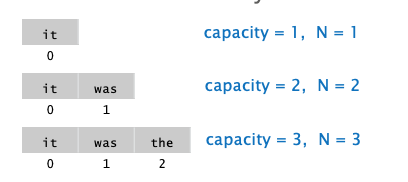
\includegraphics[width=0.5\textwidth]{Dynamic Array (Naïve).png}
    \caption{Implementation: Dynamic Array (Naïve)}
\end{figure}
Time Complexity Analysis: Each time you expand, copy all the elements of the current array into the new array. Then for the Nth expansion, copy N-1 elements. So the total number of replications is
$$1+2+3+\cdots+N=\frac{N^2+N}{2}$$
The time complexity is $O(N^2)$, which is \textbf{quadratic time}.

\subsubsection{Implementation: Dynamic Array (Better)}
Implementation Method:
\begin{itemize}
    \item The initial array size is 1.
    \item Instead of adding 1 capacity at a time, we double the capacity each time.
\end{itemize}
Time Complexity Analysis: We reduce the frequency of resize. The time complexity of the total insertion of the first N elements becomes
$$2+4+8+\cdots+N\approx O(N)$$
The time complexity is $O(N)$, which is \textbf{linear time}.
\\
Potential Problem: We don’t want a mostly empty array taking up memory. If the stack is only half full, halve the size of the array. The following illustration shows a push-pop-push-pop loop.
\begin{figure}[h]
    \centering
    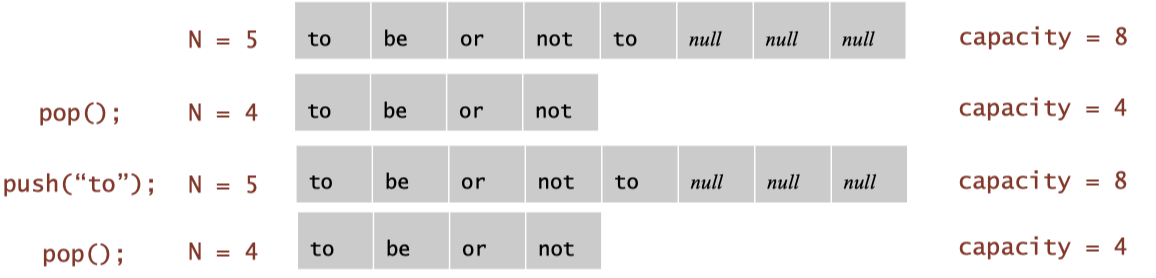
\includegraphics[width=0.9\textwidth]{push-pop-push-pop loop.png}
    \caption{Push-Pop-Push-Pop Loop}
\end{figure}
\newpage
Solution: To avoid this problem, it is common practice to set more generous shrinkage conditions, such as shrinking only when the number of elements in the stack is less than 1/4 of the capacity. For example:\\
We have capacity = 16 and the current number of elements is $N = 9$. Since $9 > 16 / 4 = 4$, there is no shrinkage.
\begin{verbatim}
Stack (capacity = 16):
[ a, b, c, d, e, f, g, h, i, _, _, _, _, _, _, _ ]
                      ↑
                      top (N = 9)
\end{verbatim}
We call \texttt{pop()} 5 times in sequence to reduce the number of elements on the stack from 9 to 4.
\begin{verbatim}
Stack after popping 5 times (capacity = 16):
[ a, b, c, d, _, _, _, _, _, _, _, _, _, _, _, _ ]
                 ↑
                 top (N = 4)
\end{verbatim}
$N = 4$, which is exactly equal to $16 / 4 = 4$, still no shrinkage (only “less than” 1/4 will shrink). So let's go ahead and pop it once.
\begin{verbatim}
Stack after popping once more:
[ a, b, c, _, _, _, _, _, _, _, _, _, _, _, _, _ ]
              ↑
              top (N = 3)
\end{verbatim}
We reduce the capacity from 16 to 8 and copy the existing elements into the new array.
\begin{verbatim}
Stack after shrinking to capacity = 8:
[ a, b, c, _, _, _, _, _ ]
           ↑
           top (N = 3)
\end{verbatim}

\section{Queue}
\subsection{Definition of Queue}
Queue stores a sequence of elements. It follows the principle of \textbf{FIFO (First In First Out)}, which means that the first element to enter the queue is the first to be removed. Queue supports 2 main operations.
\begin{itemize}
    \item \texttt{enqueue()}: Add element to tail/back.
    \item \texttt{dequeue()}: Removes and returns the element from the head/front of the queue.
\end{itemize}

\subsection{Deque: Double-Ended Queue}
For deque, elements can be inserted or deleted at either end. That means you can
\begin{itemize}
    \item Adds or removes elements from the head/front.
    \item Adds or removes elements from the tail/back.
\end{itemize}
Deque supports 4 main operations.
\begin{itemize}
    \item \texttt{addFirst()}: Insert from the front.
    \item \texttt{addLast()}: Insert from the back.
    \item \texttt{removeFirst()}: Delete from the front.
    \item \texttt{removeLast()}: Delete from the back.
\end{itemize}

\subsection{Priority Queue}
Similar to a normal queue, but \textbf{each element has a priority value}. It's not FIFO, it's whoever has the highest priority gets out of the queue first. It's like a hospital emergency room, where patients are prioritized not in order of arrival, but by the severity of their condition. There are two implementations of priority queue.
\begin{itemize}
    \item Ordered Array
    \begin{itemize}
        \item Insertions are kept in order (e.g., big-to-small sorting).
        \item The insertion operation has to find the right position (it may have to move a lot of elements).
        \item Very fast when removing elements (just remove the first one).
        \item Ideal for scenarios where there are frequent queue outs and fewer queue in.
        \item Insertion Operation Time Complexity: $O(n)$
        \item Deletion Operation Time Complexity: $O(1)$
    \end{itemize}
    \item Unordered Array
    \begin{itemize}
        \item Inserts are added directly to the end, regardless of order.
        \item Deletion scans the entire array for the highest priority element.
        \item Ideal for scenarios with frequent entries and fewer exits.
        \item Insertion Operation Time Complexity: $O(1)$
        \item Deletion Operation Time Complexity: $O(n)$
    \end{itemize}
\end{itemize}
\begin{figure}[h]
    \centering
    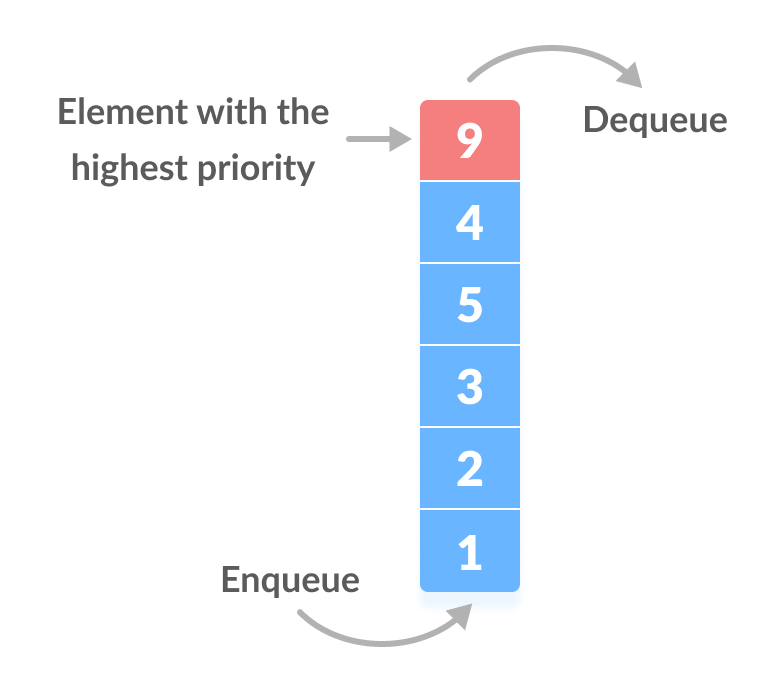
\includegraphics[width=0.5\textwidth]{Priority Queue.png}
    \caption{Priority Queue}
\end{figure}

\section{Linked List}
\subsection{Why Do We Need Linked List?}
For a traditional array, how difficult/fast are these operations?
\begin{table}[h]
    \centering
    \begin{tabular}{|l|c|c|} \hline 
          &Unordered array& Ordered array\\ \hline 
          insert&fast (just put at end)& slow (need where)\\ \hline 
          delete&slow (need to shift)& slow (need to shift)\\ \hline 
          search&slow (linear search)& fast (binary search)\\ \hline 
          resize&difficult!& difficult!\\ \hline
    \end{tabular}
    \caption{Unordered Array and Ordered Array}
    \label{tab:unordered-vs-ordered-array}
\end{table}
\\
Is it possible to have a data structure with \textbf{fast} insert, delete, and search \& easy resizing? Yes, the solution is \textbf{linked list}.

\subsection{Definition of Linked List}
A Linked List is a linear data structure consisting of a series of nodes, each containing:
\begin{itemize}
    \item Data/item
    \item Pointer/next: Points to the location of the next node in memory.
\end{itemize}
These nodes are \textbf{“linked”} together by pointers to form a \textbf{“list”}.
\begin{figure}[h]
    \centering
    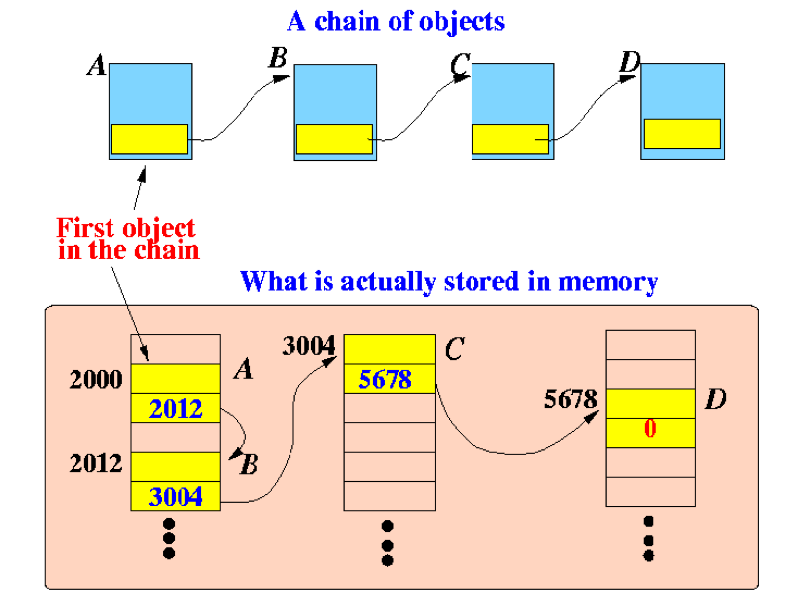
\includegraphics[width=0.8\textwidth]{linked list.png}
    \caption{Linked List}
\end{figure}
\\
A Linked List is essentially a set of node objects linked together.
\begin{verbatim}
public class Node {
    String item;   // Stored data
    Node next;     // Reference to the next node
}
\end{verbatim}
Each node is a Java object (node instance). \texttt{item} is the data it keeps for itself (e.g. “apple”, “banana”, etc.). \texttt{next} is a reference to the next node (object address). We “link” multiple node instances together to form a Linked List.
For example, the following linked list:
\begin{verbatim}
head → [ "A" |  ] → [ "B" |  ] → [ "C" | null ]
\end{verbatim}
in Java it's actually:
\begin{verbatim}
Node a = new Node();
a.item = "A";

Node b = new Node();
b.item = "B";
a.next = b;   // A → B

Node c = new Node();
c.item = "C";
b.next = c;   // B → C

c.next = null; // C is the last node.
\end{verbatim}
Array vs. Linked List:
\begin{table}[h]
    \centering
    \begin{tabular}{|c|c|} \hline 
          Array& Linked List\\ \hline 
          Store elements contiguously in memory& Not stored contiguously in memory\\ \hline 
          Fixed size& Dynamic size\\ \hline 
          Supports direct index access& No indexed access\\ \hline 
          & Some memory overhead to store references\\ \hline
    \end{tabular}
    \caption{Array \& Linked List}
    \label{tab:array-vs-linked-list}
\end{table}

\subsection{Linked List Operations}
\begin{verbatim}
public class SimpleLinkedList {

    // Define the node class for the linked list
    static class Node {
        String item;
        Node next;

        Node(String item) {
            this.item = item;
            this.next = null;
        }
    }

    // Head node of the linked list
    private Node head;

    public SimpleLinkedList() {
        head = null;
    }

    // ===============================
    // 1. Build the list (add elements at the end)
    // ===============================
    public void buildList(String[] items) {
        for (String item : items) {
            insertAtEnd(item);
        }
    }

    // ===============================
    // 2. Traverse the list
    // ===============================
    public void traverse() {
        Node current = head;
        System.out.print("List: ");
        while (current != null) {
            System.out.print(current.item + " → ");
            current = current.next;
        }
        System.out.println("null");
    }

    // ===============================
    // 3. Search for a given item (returns true/false)
    // ===============================
    public boolean search(String key) {
        Node current = head;
        while (current != null) {
            if (current.item.equals(key)) {
                return true;
            }
            current = current.next;
        }
        return false;
    }

    // ===============================
    // 4. Insert an element (at the beginning)
    // ===============================
    public void insertAtBeginning(String item) {
        Node newNode = new Node(item);
        newNode.next = head;
        head = newNode;
    }

    // Insert an element (at the end)
    public void insertAtEnd(String item) {
        Node newNode = new Node(item);
        if (head == null) {
            head = newNode;
            return;
        }
        Node current = head;
        while (current.next != null) {
            current = current.next;
        }
        current.next = newNode;
    }

    // ===============================
    // 5. Delete an element (from the beginning)
    // ===============================
    public void deleteFromBeginning() {
        if (head != null) {
            head = head.next;
        }
    }

    // Delete an element (from the end)
    public void deleteFromEnd() {
        if (head == null || head.next == null) {
            head = null;
            return;
        }
        Node current = head;
        while (current.next.next != null) {
            current = current.next;
        }
        current.next = null;
    }

    // Delete a node by value (key)
    public void deleteByKey(String key) {
        if (head == null) return;

        // If the node to be deleted is the head
        if (head.item.equals(key)) {
            head = head.next;
            return;
        }

        Node current = head;
        while (current.next != null && !current.next.item.equals(key)) {
            current = current.next;
        }

        // If the target node is found
        if (current.next != null) {
            current.next = current.next.next;
        }
    }

    // ========== Main method for testing ==========
    public static void main(String[] args) {
        SimpleLinkedList list = new SimpleLinkedList();

        // Build a list from array
        list.buildList(new String[]{"A", "B", "C"});
        list.traverse();  // A → B → C → null

        // Insert test
        list.insertAtBeginning("START");
        list.insertAtEnd("END");
        list.traverse();  // START → A → B → C → END → null

        // Search test
        System.out.println("Search B: " + list.search("B"));  // true
        System.out.println("Search Z: " + list.search("Z"));  // false

        // Deletion tests
        list.deleteFromBeginning();  // Delete START
        list.traverse();

        list.deleteFromEnd();        // Delete END
        list.traverse();

        list.deleteByKey("B");       // Delete B
        list.traverse();
    }
}
\end{verbatim}

\subsection{Types of Linked Lists}
\subsubsection{Double-Ended (Singly) Linked List}
Also keep a reference to the last element of the list.
\begin{itemize}
    \item What happens when the list is empty? first = last = null
    \item What happens when there is one element? first = last = that one element
\end{itemize}
\subsubsection{Doubly Linked List}
Every node has a next pointer and a previous pointer.
\begin{figure}[h]
    \centering
    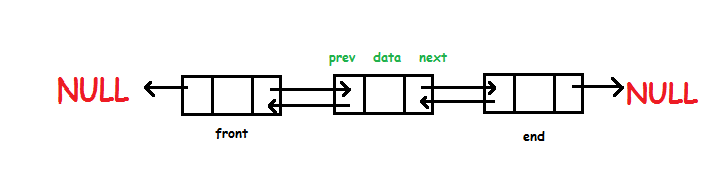
\includegraphics[width=0.8\textwidth]{Doubly Linked List.png}
    \caption{Doubly Linked List}
\end{figure}
\subsubsection{Circular Linked List}
Instead of the last node’s next field being null, point back to the first node.
\begin{figure}[h]
    \centering
    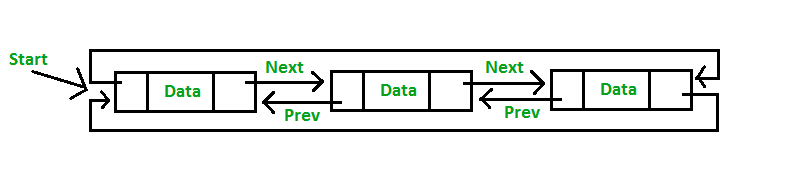
\includegraphics[width=0.8\textwidth]{Circular Linked List.png}
    \caption{Circular Linked List}
\end{figure}

\subsection{Stacks Linked List Implementation}
Implementation: using a unidirectional linked list to build a stack.
\subsubsection{Defining Linked List}
\begin{verbatim}
private Node first = null;
\end{verbatim}
\texttt{first} is the head of the chain and the top of the stack.
\begin{verbatim}
private class Node {
    Item item;
    Node next;
}
\end{verbatim}
Each node contains a data \texttt{item} and a pointer to the next node \texttt{next}.

\subsubsection{\texttt{push(Item item)}: Adding Element to Top of Stack}
\begin{verbatim}
public void push(Item item) {
    Node oldfirst = first;
    first = new Node();
    first.item = item;
    first.next = oldfirst;
}
\end{verbatim}
We create a new node and place it at the head of the linked list. What was the top of the stack becomes the \texttt{.next} of the new node.

\subsubsection{\texttt{pop()}: Removing Element from Top of Stack}
\begin{verbatim}
public Item pop() {
    Item item = first.item;
    first = first.next;
    return item;
}
\end{verbatim}
Take out the contents of the header node directly, and then have \texttt{first} point to the next node. The original first node is “dropped”.

\subsection{Queues Linked List Implementation}
Implementation: using a double-ended singly linked list to build a queue.
\subsubsection{Defining Linked List}
\begin{verbatim}
private Node<Item> first, last;
\end{verbatim}
\texttt{first} points to the front - the place where you want to get out of the queue. \texttt{last} points to the back - place to enter the queue. This is in line with the \textbf{FIFO (First-In-First-Out)} queuing feature.

\subsubsection{\texttt{enqueue(Item item)}: Getting in the Queue (Adding at the End)}
\begin{verbatim}
public void enqueue(Item item) {
    Node oldlast = last;
    last = new Node();          // Creating a new node
    last.item = item;
    last.next = null;
    
    if (isEmpty())
        first = last;
        // The queue is empty and the new node is both head and tail
    else
        oldlast.next = last;
        // Attach the new node to the original tail node
}
\end{verbatim}

\subsubsection{\texttt{dequeue()}: Out of Queue (Head Removed)}
\begin{verbatim}
public Item dequeue() {
    Item item = first.item;
    first = first.next;
    // Moving the head pointer forward
    if (isEmpty())
        last = null;
        // If the queue becomes empty, clear the tail pointer.
    return item;
}
\end{verbatim}

\part{Algorithms and Sorting}

\section{Algorithm Analysis}
\subsection{What Is A Good Algorithm?}
There are two criteria for the answer:
\begin{itemize}
    \item Low Running Time: This means that the algorithm executes fast. We usually measure this by \textbf{Time Complexity (Big-O representation)}.
    \item Efficient Usage of Space (Memory): Use as little extra space as possible to minimize memory footprint \textbf{(Space Complexity)}.
\end{itemize}

\subsection{Loop Analysis}
Most operations in a program are done by loops to iterate through the input data. Loops are often a major determinant of runtime, especially when you are dealing with large amounts of data (e.g. arrays, lists, etc.).

\subsubsection{Total Cost}
How to Calculate the Time Complexity (Total Cost) of A Loop?
\begin{itemize}
    \item Count how many statements there are in the loop body (usually assignments, additions, function calls, etc.).
    \item Analyze how many times the loop is executed (usually related to $n$, $n^2$, etc.).
    \item Multiply the two: $$\text{Number of Statements} \times \text{Number of Executions} =\text{Total Cost}$$
\end{itemize}
Example 1:
\begin{verbatim}
double sum = 0.0;
for (int i = 0; i < n; i++) {
    sum += array[i];
}
\end{verbatim}
In this example,
$$\text{Number of Statements} \times \text{Number of Executions} = 1 \times n = n = \text{Total Cost}$$
Example 2:
\begin{verbatim}
for (int i = 0; i < n; i++) {
    for (int j = 0; j < n; j++) {
        System.out.println(i + ", " + j);
    }
}
\end{verbatim}
In this example,
$$\text{Number of Statements} \times \text{Number of Executions} = 1 \times n \times n = n^2 = \text{Total Cost}$$
If we encounter nested loops, we use \textbf{the number of outer loops multiplied by the number of inner loops to equal the total number of executions}.\\
Example 3:
\begin{verbatim}
for (int i = 0; i < n; i++) {
    for (int j = 0; j < i; j++) {
        System.out.println(i + ", " + j);
    }
}
\end{verbatim}
In this example, the number of statements is 1 and the number of executions of the inner loop grows with $i$.
\begin{itemize}
    \item When $i = 0$ and $j < 0$, it is executed $0$ times.
    \item When $i = 1$ and $j < 1$, it is executed $1$ times.
    \item When $i = 2$ and $j < 2$, it is executed $2$ times.
    \item ...
    \item When $i = n-1$ and $j < n-1$, it is executed $n-1$ times.
\end{itemize}
So the total number of executions is:
$$0 + 1 + 2 + ... + (n-1) = n(n-1)/2$$
In the end, the total cost is:
$$\text{Total Cost} = 1 \times [0 + 1 + 2 + ... + (n-1)] = n(n-1)/2$$
Example 4:
\begin{verbatim}
for (int i = 0; i < n; i++) {
    for (int j = i; j < n; j++) {
        System.out.println(i + ", " + j);
    }
}
\end{verbatim}
In this example, the number of statements is 1 and the number of inner loop executions depends on $i$.
\begin{itemize}
    \item When $i = 0$: $j$ goes from $0$ to $n-1$; it execute $n$ times.
    \item When $i = 1$: $j$ goes from $1$ to $n-1$; it execute $n-1$ times.
    \item ...
    \item When $i = n-1$: $j$ goes from $n-1$ to $n-1$; it execute $1$ times.
\end{itemize}
So the total number of executions is:
$$n + (n-1) + (n-2) + ... + 1 = n(n+1)/2$$
In the end, the total cost is:
$$\text{Total Cost} = 1 \times (n(n+1)/2) = n(n+1)/2$$

\subsubsection{Big O Representation}
Method 1:
\begin{enumerate}
    \item Derive the cost function $f(n)$ of your algorithm. Example: $3n^2 + 5n + 10$.
    \item Throw away lower-order terms [tilde notation]. Example: $~3n^2$.
    \item Drop constant factors [Big-Oh notation]. Example: $O(n^2)$.
\end{enumerate}
Method 2: Use the mnemonic.\\
Each loop has a corresponding update expression. For example, for the following loop, the update expression is \texttt{i++}.
\begin{verbatim}
double sum = 0.0;
for (int i = 0; i < n; i++) {
    sum += array[i];
}
\end{verbatim}
We can derive big O by using the following mnemonic in combination with the update expression.
\begin{enumerate}
    \item For a single-level loop, it is $O(n)$ if the update expression is addition or subtraction, and $O(logn)$ if the update expression is multiplication or division.
    \item For nested loops, if the inner loop depends on the outer loop.
    \begin{enumerate}
        \item The outer loop is additive and subtractive, and the inner loop is also additive and subtractive, with a time complexity of $O(n^2)$.
        \item The outer loop is multiplication and division and the inner loop is addition and subtraction with $O(n)$ time complexity.
        \item The outer loop is addition and subtraction and the inner loop is multiplication and division with a time complexity of $O(n logn)$.
        \item The outer loop is multiplication and division and the inner loop is also multiplication and division with a time complexity of $O((log n)^2)$.
        \item In summery, in most cases, the time complexity of a nested loop is equal to the product of the time complexities of the inner and outer loops, except when the inner loop's bound depends on the outer loop and the outer loop grows multiplicatively (e.g., \texttt{i *= 2}) while the inner loop grows additively (e.g., \texttt{j++}).
    \end{enumerate}
    \item For nested loop, if inner loop does not depend on outer loop, we directly multiply inner time complexity by outer time complexity to equal the overall time complexity.
    \item If two loops are sequential (i.e., not nested), the total time complexity is the maximum of the two. $O(n) > O((\log n)^2) > O(\log n)$.
\end{enumerate}
Example 1:
\begin{verbatim}
double sum = 0.0;
for (int i = 0; i < n; i++) {
    sum += array[i];
}
\end{verbatim}
It is single-level loop; update expression is plus; time complexity is $O(n)$.\\
Example 2:
\begin{verbatim}
for (int i = 0; i < n; i++) {
    for (int j = i; j < n; j++) {
        System.out.println(i + ", " + j);
    }
}
\end{verbatim}
It is nested loop; update expression is plus for inner and outer loop; time complexity is $O(n^2)$.

\section{Simple Sorting}
\subsection{Bubble Sort}
\subsubsection{Algorithm}
The essence of bubble sort is to push large elements backward through multiple rounds of swapping.
\begin{itemize}
    \item We traverse the entire list of data one at a time.
    \begin{itemize}
        \item If two neighboring elements are found in the wrong order (e.g., the former is larger than the latter), swap them.
    \end{itemize}
    \item In each round, the current largest element “bubbles up” to the end.
    \item The next round simply traverses up to just before the last position of the previous round, as it is already lined up.
    \item Repeat this process until all elements are ordered.
\end{itemize}
Here is the code of bubble sort.
\begin{verbatim}
void bubbleSort(int arr[])
{
    int n = arr.length;
    for (int i = 0; i < n-1; i++)
        for (int j = 0; j < n-i-1; j++)
            if (arr[j] > arr[j+1])
            {
                // swap temp and arr[i]
                int temp = arr[j];
                arr[j] = arr[j+1];
                arr[j+1] = temp;
            }
}
\end{verbatim}
\subsubsection{Example of Bubble Sort}
The original array is 51428.
\begin{enumerate}
    \item Round 1: 14258.
    \begin{enumerate}
        \item First of all, the algorithm compare the first two element and swaps since $5>1$. $$(5,1,4,2,8)---(1,5,4,2,8)$$
        \item Since $5>4$, we swap 5 and 4. $$(1,5,4,2,8)---(1,4,5,2,8)$$
        \item Since $5>2$, we swap 5 and 2. $$(1,4,5,2,8)---(1,4,2,5,8)$$
    \end{enumerate}
    \item Round 2: 12458.
    \begin{enumerate}
        \item First of all, the algorithm compare the first two element and do not swap. Then, the algorithm compare 4 and 2. The algorithm swap 4 and 2 since $4>2$. $$(1,4,2,5,8)---(1,2,4,5,8)$$
        \item Now, the array is already sorted, but our algorithm does not know if it is completed. The algorithm needs one whole pass without any swap to know it is sorted.
    \end{enumerate}
    \item Round 3: 12458.
\end{enumerate}

\subsection{Selection Sort}
\subsubsection{Algorithm}
The essence of selection sort is to keep swapping the smallest element with the first of the parts that are not yet sorted.
\begin{itemize}
    \item Scan from left to right, keeping the int i as the integer of the smallest item you’ve seen so far.
    \item After the scan, move the element at i to the left-most position.
    \item Repeat, starting from the second element this time.
    \item Then the third element…
\end{itemize}
Here is the code of selection sort.
\begin{verbatim}
public static void sort(Comparable[] a) {
    int N = a.length;
    for (int i = 0; i < N; i++) {
        int min = i;
        for (int j = i+1; j < N; j++)
            if (less(a[j], a[min]))
                min = j;  // update minimum index
        exch(a, i, min);
    }
}
\end{verbatim}
\subsubsection{Example of Selection Sort}
The original array is 51428.
\begin{enumerate}
    \item Round 1: 15428.
    \begin{enumerate}
        \item The smallest is 1. We swap 1 and the first of the array (5).
    \end{enumerate}
    \item Round 2: 12458
    \begin{enumerate}
        \item The smallest is 2. We swap 2 and the first of the unsorted part of the array (5).
    \end{enumerate}
\end{enumerate}

\subsection{Insertion Sort}
\subsubsection{Algorithm}
The essence of insertion sort is to keep shifting a number forward until it gets to the right place.
\begin{itemize}
    \item Partition the elements into two regions.
    \item Assume the left side is partially sorted. Elements on the left side are in a sorted order, but not necessarily in their final positions.
    \item For each remaining element on the right side, insert the element where it belongs on the left side.
    \item Repeat until done…
\end{itemize}
Here is the code of insertion sort.
\begin{verbatim}
public static void sort(Comparable[] a) {
    int N = a.length;
    for (int i = 0; i < N; i++)
        for (int j = i; j > 0; j--)
            if (less(a[j], a[j-1]))
                exch(a, j, j-1);
            else break;
}
\end{verbatim}
\subsubsection{Example of Insertion Sort}
The original array is 51428.
\begin{itemize}
    \item Round 1: $[5 | 1 4 2 8]$ (no swaps)
    \item Round 2: $[1 5 | 4 2 8]$ (1 swap)
    \item Round 3: $[1 4 5 | 2 8]$ (1 swap)
    \item Round 4: $[1 2 4 5 | 8]$ (2 swaps)
    \item Round 5: $[1 2 4 5 8]$ (no swaps)
\end{itemize}

\section{Merge Sort and Quick Sort}
\subsection{Algorithm of Merge Sort}
Merge Sort splits an array in two, recursively sorts the left and right parts, and then merges them into a single ordered array. It is essentially the logic of \textbf{divide and conquer}.
\begin{itemize}
    \item Divide the list into two halves
    \item Sort each half
    \item Merge each half in sorted order
\end{itemize}
\subsection{Example of Merge Sort}
The original array is $[38,27,43,3,9,82,10]$.
\begin{itemize}
    \item Stage 1 Split Phase: Keep “halving” the array until there is only one element left in each subarray (individual elements are naturally ordered).
    \begin{itemize}
        \item 1st layer split: split into left and right halves.
        $$[38,27,43,3] \text{and} [9,82,10]$$
        \item 2nd layer split: continue to divide.
        $$[38,27], [43,3], [9,82], [10]$$
        \item 3rd layer split: final split into individual elements.
        $$[38],[27],[43],[3],[9],[82],[10]$$
    \end{itemize}
    \item Stage 2 Merge Phase: Starting at the bottom, two by two, they are merged into ordered subarrays until they are finally merged into a complete ordered array.
    \begin{itemize}
        \item 1st layer merge:
        $$[27,38], [3,43], [9,82], [10]$$
        \item 2nd layer merge:
        $$[3,27,38,43], [9,10,82]$$
        \item 3rd layer merge:
        $$[3,9,10,27,38,43,82]$$
    \end{itemize}
\end{itemize}

\subsection{Some Facts about Merge Sort}
\begin{itemize}
    \item Algorithm Type: Divide and Conquer
    \item Recursive or Not: This is recursive (keep splitting the array + merging).
    \item Whether to Sort In-place: No, additional memory space (auxiliary array) is required.
    \item Average Time Complexity: $O(n logn)$
    \item Best Case Time Complexity: $O(n logn)$
    \item Worst Case Time Complexity: $O(n logn)$
\end{itemize}

\subsection{Algorithm of Quick Sort}
Quick Sort selects a pivot, then puts the one smaller than the pivot on the left side of the pivot, and the one larger than the pivot on the right side of the pivot, with constant recursion, to complete the sort. It is essentially the logic of \textbf{divide and conquer}.
\begin{itemize}
    \item Shuffle the array: avoiding arrays that are already ordered or reverse-ordered.
    \item Partition so that for some j:
    \begin{itemize}
        \item entry a[j] is in place.
        \item no larger entry to the left of j.
        \item no smaller entry to the right of j.
    \end{itemize}
    \item Recursively sort.
\end{itemize}

\subsection{Example of Quick Sort}
The original array is $[38,27,43,3,9,82,10]$.
\begin{itemize}
    \item Stage 1: Overall sorting and pivot is 10. We put anything less than or equal to 10 on the left and anything greater than on the right.
    $$[3,9,10,38,27,82,43]$$
    \item Stage 2: Quick sort the left $[3,9]$ and pivot is 9. Remain unchanged.
    $$[3,9]$$
    \item Stage 3: Quick sort the right $[38,27,82,43]$ and pivot is 43.
    $$[38,27,43,82]$$
    \item Stage 4: Quick sort the left $[38,27]$ and pivot is 27.
    $$[27,38]$$
    \item Stage 5: Combine all the subarray and the pivots.
    $$[3,9,10,27,38,43,82]$$
\end{itemize}

\subsection{Some Facts about Quick Sort}
\begin{itemize}
    \item Algorithm Type: Divide and Conquer
    \item Recursive or Not: This is recursive (sorting subarrays by recursion).
    \item Whether to Sort In-place: Yes, no additional arrays are needed (except for the recursive stack).
    \item Average Time Complexity: $O(n logn)$
    \item Best Case Time Complexity: $O(n logn)$
    \item Worst Case Time Complexity: $O(n^2)$ when pivot is extremely unbalanced (e.g. array is sorted + first pivot is selected).
    \item Suitability for Big Data Sorting: Usually very fast, faster than mergesort in practice.
    \item How to avoid the Worst Case Scenario: Using randomized pivot to shuffle the array.
\end{itemize}

\section{Sorting Code Explanation and Time Complexity}
\subsection{Simple Sort Code}
\begin{verbatim}
public class SortingAlgorithms {

    // Bubble Sort
    public static void bubbleSort(int[] arr) {
        for (int i = 0; i < arr.length - 1; i++) {
            for (int j = 0; j < arr.length - 1 - i; j++) {
                if (arr[j] > arr[j + 1]) {
                    int temp = arr[j];
                    arr[j] = arr[j + 1];
                    arr[j + 1] = temp;
                }
            }
        }
    }

    // Selection Sort
    public static void selectionSort(int[] arr) {
        for (int i = 0; i < arr.length - 1; i++) {
            int minIndex = i;
            for (int j = i + 1; j < arr.length; j++) {
                if (arr[j] < arr[minIndex]) {
                    minIndex = j;
                }
            }
            int temp = arr[i];
            arr[i] = arr[minIndex];
            arr[minIndex] = temp;
        }
    }

    // Insertion Sort
    public static void insertionSort(int[] arr) {
        for (int i = 1; i < arr.length; i++) {
            int key = arr[i];
            int j = i - 1;
            while (j >= 0 && arr[j] > key) {
                arr[j + 1] = arr[j];
                j--;
            }
            arr[j + 1] = key;
        }
    }
}
\end{verbatim}

\subsection{Merge Sort Code}
\begin{verbatim}
public class MergeSort {

    // Main function: the entry point of the program, used to demonstrate
    // the Merge Sort effect.
    public static void main(String[] args) {
        // Create an integer array (to be sorted)
        Integer[] array = {9, 3, 7, 1, 6, 8, 2, 5, 4};

        // Print the array before sorting.
        System.out.println("Before sorting:");
        printArray(array);

        // Call the mergesort method to sort the array.
        mergesort(array);

        // Print the sorted array.
        System.out.println("After sorting:");
        printArray(array);
    }

    // Public entry method for Merge Sort
    public static void mergesort(Comparable[] a) {
        // Create an auxiliary array of the same size as the original
        // array for temporary data storage during merging
        Comparable[] aux = new Comparable[a.length];

        // Call the recursive sort method to start sorting the entire
        // array.
        sort(a, aux, 0, a.length - 1);
    }

    /**
     * Recursive sort function: sorting the interval a[lo..hi]
     *
     * @param a   original array
     * @param aux auxiliary arrays for storing data during merge operations
     * @param lo  starting index of the current subarray
     * @param hi  ending index of the current subarray
     */
    private static void sort(Comparable[] a, Comparable[] aux, int lo, int hi) {
        // When the subarray contains only one element or is empty, it is
        // returned directly (base case)
        if (hi <= lo) return;

        // Calculate the middle position for splitting the array
        int mid = lo + (hi - lo) / 2;

        // Recursive sort on the left half a[lo..mid]
        sort(a, aux, lo, mid);

        // Recursive sort on right half a[mid+1..hi]
        sort(a, aux, mid + 1, hi);

        // Merge left and right parts (a[lo..mid] with a[mid+1..hi])
        merge(a, aux, lo, mid, hi);
    }

    /**
     * Merge two sorted subarrays a[lo..mid] and a[mid+1..hi].
     */
    private static void merge(Comparable[] a, Comparable[] aux, int lo,
    int mid, int hi) {
        // Step 1: Copy all elements of a[lo..hi] into the auxiliary array
        // aux
        for (int k = lo; k <= hi; k++) {
            aux[k] = a[k];
        }

        // i points to the starting position of the left half, j points to
        // the starting position of the right half
        int i = lo, j = mid + 1;

        // Step 2: Perform a merge, placing the smaller elements in order
        // into the original array a
        for (int k = lo; k <= hi; k++) {
            if (i > mid) {
                // If the left half is exhausted, take the right half of
                // the element directly
                a[k] = aux[j++];
            } else if (j > hi) {
                // If the right half is exhausted, take the left half of
                // the element directly
                a[k] = aux[i++];
            } else if (less(aux[j], aux[i])) {
                // If the right element is smaller, then take the right
                // element and put it into a[k]
                a[k] = aux[j++];
            } else {
                // Otherwise take the left element and put it into a[k]
                a[k] = aux[i++];
            }
        }
    }
}
\end{verbatim}

\subsection{Quick Sort Code}
\begin{verbatim}
// Quick Sort implementation in basic Java
public class QuickSort {

    // Main method to demonstrate quick sort
    public static void main(String[] args) {
        int[] array = {9, 3, 7, 1, 6, 8, 2, 5, 4};

        System.out.println("Before sorting:");
        printArray(array);

        quickSort(array, 0, array.length - 1);

        System.out.println("After sorting:");
        printArray(array);
    }

    // Quick Sort function
    public static void quickSort(int[] arr, int low, int high) {
        if (low < high) {
            int pivotIndex = partition(arr, low, high);
            quickSort(arr, low, pivotIndex - 1);  // Sort left part
            quickSort(arr, pivotIndex + 1, high); // Sort right part
        }
    }

    // Partition the array and return pivot index
    private static int partition(int[] arr, int low, int high) {
        int pivot = arr[high]; // Choose the last element as pivot
        int i = low - 1;       // Index of smaller element

        for (int j = low; j < high; j++) {
            if (arr[j] <= pivot) {
                i++;
                swap(arr, i, j); // Swap if element is <= pivot
            }
        }

        swap(arr, i + 1, high); // Move pivot to correct position
        return i + 1;
    }

    // Swap two elements in array
    private static void swap(int[] arr, int i, int j) {
        int temp = arr[i];
        arr[i] = arr[j];
        arr[j] = temp;
    }

    // Utility function to print array
    private static void printArray(int[] arr) {
        for (int num : arr) {
            System.out.print(num + " ");
        }
        System.out.println();
    }
} 
\end{verbatim}

\subsection{Time Complexity of Sorting Method}
\begin{table}[h!]
\centering
\renewcommand{\arraystretch}{1.3}
\begin{tabular}{|l|c|c|c|}
\hline
\textbf{Sorting Method} & \textbf{Best Case} & \textbf{Average Case} & \textbf{Worst Case} \\
\hline
Bubble Sort      & $O(n)$           & $O(n^2)$         & $O(n^2)$         \\
Selection Sort   & $O(n^2)$         & $O(n^2)$         & $O(n^2)$         \\
Insertion Sort   & $O(n)$           & $O(n^2)$         & $O(n^2)$         \\
\hline
Merge Sort       & $O(n \log n)$    & $O(n \log n)$    & $O(n \log n)$    \\
\quad -- divide (compute mid) & $O(1)$ per level & $O(1)$ per level & $O(1)$ per level \\
\quad -- sort (recursive calls) & $\log n$ levels & $\log n$ levels & $\log n$ levels \\
\quad -- merge step & $O(n)$ per level & $O(n)$ per level & $O(n)$ per level \\
\hline
Quick Sort       & $O(n \log n)$    & $O(n \log n)$    & $O(n^2)$         \\
\quad -- partition & $O(n)$         & $O(n)$           & $O(n)$           \\
\quad -- sort (recursive calls) & $\log n$ levels & $\log n$ levels & $n$ levels (degenerate) \\
\hline
\end{tabular}
\caption{Time complexity breakdown of five sorting algorithms, including component analysis for Merge Sort and Quick Sort}
\end{table}
\end{document}